% vim: tw=80 noai
\documentclass[normaltoc,capchap,capsec,times]{abnt}
\usepackage[utf8x]{inputenc}
\usepackage[T1]{fontenc}
\usepackage[brazil]{babel}
\usepackage[alf]{abntcite}
\usepackage[ordem=alf]{tabela-simbolos}
\usepackage{url}
\usepackage[pdftex]{graphicx}
\usepackage{listings}
\usepackage{verbatim}
\usepackage{subfigure}
\usepackage{multicol}
\usepackage{multirow}
\usepackage{framed}
%\usepackage{algorithm2e}
\usepackage{amssymb, amsmath}
\usepackage{listings}

\def\lstlistingname{Listagem}

%%%%%%%%%%%%%%%%%%%%%%%%%%%%%%%%%%%%%%%%%%%%%%%%%%%%
% Dados da monografia
%%%%%%%%%%%%%%%%%%%%%%%%%%%%%%%%%%%%%%%%%%%%%%%%%%%%

\newcommand{\meunome}{Aline Duarte Bessa}
\newcommand{\meutitulo}{Classificação de documentos de acordo com pontos de vista sobre um tema}
\newcommand{\meusubtitulo}{Aspectos teóricos e práticos}
\newcommand{\meuano}{2010}
\newcommand{\meuorientador}{Orientador: Alexandre Tachard Passos}
\newcommand{\meucoorientador}{Co-orientador: Luciano Porto Barreto}

%%%%%%%%%%%%%%%%%%%%%%%%%%%%%%%%%%%%%%%%%%%%%%%%%%%%

%% O comando \obs aqui definido permite que o autor faca anotacoes na
%% monografia que aparecem no PDF gerado. Para ativar o comando, descomente
%% a primeira linha e comente a segunda.
%% Exemplo de uso: \obs{Preciso melhorar este parágrafo...}

%\newcommand{\obs}[1]{\underline{\textbf{OBSERVAÇÃO}}: \emph{#1}}
\newcommand{\obs}[1]{}

\def\ordfem{\mbox{\raise .35em \hbox{\underline{\scriptsize a}\ }}}
\def\ordmasc{\mbox{\raise .35em \hbox{\underline{\scriptsize o}\ }}}
\def\profa{Prof\ordfem.}

%%%%%%%%%%%%%%%%%%%%%%%%%%%%%%%%%%%%%%%%%%%%%%%%%%%%

\begin{document}

% Capa com Brasão

\begin{titlepage}
   \begin{center}
      %logotipo
               
\includegraphics{brasaoUFBA} \\
  %\vspace{0.7in}
              \centering{ 
        \bf{
        \LARGE{
    \uppercase{UNIVERSIDADE FEDERAL DA BAHIA} \\
        }
        \Large {
                    \uppercase{INSTITUTO DE MATEMÁTICA} \\
        }
                   \large {
                       \uppercase{DEPARTAMENTO DE CIÊNCIA DA COMPUTAÇÃO} \\
                  }
              } }
   \end{center}
   \vfill
   \begin{center}
       \bf{
       \large{\uppercase{\meunome}  \\  }
       }
   \end{center}
   \vspace{0.2in}
   \begin{center}
       \bf{
         \LARGE{ \uppercase{\meutitulo} } \\
         \Large{ \uppercase{\meusubtitulo} }
         \obs{\\ \Large{Esta versão da monografia contém comentários do autor.
          Para removê-los, redefina o comando LaTeX \texttt{obs}.}}
       }
   \end{center}

   \vfill
   \hspace{\stretch{1}}
   \vfill
   \begin{center}
      \normalsize{
          Salvador \\
          \meuano
       }
   \end{center}

\end{titlepage}

%comando abaixo cria uma capa redundante, mas como a capa com brasão foi 
% feita 'manualmente', não faz sentido usar este comando:
%\capa



%\folhaderosto
% o comando acima foi comentado para não criar uma folha de 
% rosto redundante, já que ela feita 'manualmente' abaixo

\begin{titlepage}
 \vfill
 \begin{center}
   {\large \uppercase{ \bf{ \meunome\ } } } \\[7cm]
   {\Huge \uppercase{ \bf{ \meutitulo\ } } }\\[1cm]
   \vfill
   \hspace{.45\textwidth} % posicionando a minipage
   \begin{minipage}{.5\textwidth}
     \begin{espacosimples}
       \bf{
  Monografia apresentada ao Curso de graduação em Ciência da Computação, 
  Departamento de Ciência da Computação, Instituto de Matemática,  Universidade Federal da 
  Bahia, como requisito parcial para obtenção do grau de Bacharel em  Ciência da Computação. \\ 
       }      
     \end{espacosimples}
     \begin{espacosimples}    
       \meuorientador \\
       \meucoorientador
     \end{espacosimples}
   \end{minipage}
   \vfill
   Salvador \\
   \meuano
 \end{center}
\end{titlepage}

\chapter*{Agradecimentos}

À UFBA, por viabilizar esta monografia.

A meu orientador e amigo Alexandre Passos, por me ajudar a definir o tema, me motivar e participar ativamente de todo o processo.

A meu co-orientador Luciano Porto, pelas sugestões e por acompanhar esta monografia do começo ao fim.

À minha mãe, por ser meu baluarte durante todos esses anos. A meu pai, por me fazer ver tudo de forma mais simples.

A Andrea Bessa e Lucas Cunha, jornalistas que me ajudaram a selecionar bons \emph{sites} de política brasileira, fundamentais para essa monografia. E a Marcelo Pessoa, por gostar tanto de política e analisar esse trabalho sob a ótica de alguém não-envolvido.

A todos os meus amigos, pelos momentos maravilhosos nos fins de semana e compreensão com meus sumiços.



\begin{resumo}
A classificação de documentos de acordo com seus pontos de vista sobre um tema é um tópico de pesquisa que vem recebendo atenção crescente. Dado um conjunto de documentos sobre a política dos Estados Unidos, por exemplo, esse tipo de classificação pode ser empregado 
para identificar quais deles defendem o ponto de vista \emph{liberal} e quais defendem o ponto de vista 
\emph{conservador}. Esse tipo de classificação colabora com a análise de documentos argumentativos, especialmente quando não é possível lê-los um por  um. Devido ao caráter desses documentos, esse tipo de classificação pode fazer parte de estudos interdisciplinares, envolvendo áreas como Ciência Política e Comunicação. 

Diante disso, essa monografia apresenta uma revisão de trabalhos que tratam desse tópico, indicando quais são os principais classificadores utilizados, quais aspectos dos documentos podem ser explorados na identificação de seus pontos de vista, dentre outros aspectos associados a esse tópico de pesquisa. Em seguida, é feito um estudo de caso envolvendo documentos sobre a política brasileira escritos em 2010, ano de eleição presidencial. Eles são classificados de acordo com os pontos de vista \emph{pró-oposição} e \emph{pró-situação}, e as palavras mais enfatizadas por cada ponto de vista também são discutidas. 


%    Diante disso, estudos com o intuito de extrair opiniões e pontos de vista da Web, e interpretá-
%los automaticamente, tornaram-se mais frequentes na área de Ciência da Computação. Juntos,

%, que visa a separar documentos de acordo com seus diferentes posicionamentos sobre um tema


%e outros aspectos associados a 

\textbf{Palavras-chave:}
Mineração de opinião,
classificação, 
política brasileira,
ponto de vista.
\end{resumo}

% O abstract e' opcional.
\begin{abstract}
Documents classification according to their viewpoints is a research topic that has been receiving a growing attention. Given a set of documents about the United States politics, for example, this kind of classification may be useful to identify those that defend a \emph{liberal} viewpoint and those that defend a \emph{conservative} one. This kind of classification is helpful in analyzing argumentative documents, specially when it is not possible to read them one by one. Due to the content of these documents, this kind of classification may be part of interdisciplinary studies, involving areas such as Political Sciences or Communication.

In the view of this, this monograph presents a review of papers that discuss this topic, indicating which classifiers are the most used, which aspects of the documents may be exploited in the identification of their viewpoints, among other aspects associated to this research topic. After that, a case study is conducted, involving documents about brazilian politics written in 2010, year of brazilian presidential election. They are classified according to the \emph{pro-situation} and \emph{pro-opposition} viewpoints, and the words that are more emphasized by each viewpoint are also discussed.     

%A classificação de documentos de acordo com seus pontos de vista sobre um tema é um tópico de pesquisa que vem recebendo atenção crescente. Dado um conjunto de documentos sobre a política dos Estados Unidos, por exemplo, esse tipo de classificação pode ser empregado 
%para identificar quais deles defendem o ponto de vista \emph{liberal} e quais defendem o ponto de vista 
%\emph{conservador}. Esse tipo de classificação colabora com a análise de documentos argumentativos, especialmente em cenários nos quais não é possível lê-los um a um. Devido ao caráter desses documentos, esse tipo de classificação pode fazer parte de estudos interdisciplinares, envolvendo áreas como Ciência Política e Comunicação. 

%Diante disso, essa monografia apresenta uma revisão de trabalhos que tratam desse tópico, indicando quais são os principais classificadores utilizados, quais aspectos dos documentos podem ser explorados na identificação de seus pontos de vista, dentre outros aspectos associados a esse tópico de pesquisa. Em seguida, é feito um estudo de caso envolvendo documentos sobre a política brasileira escritos em 2010, ano de eleição presidencial. Eles são classificados de acordo com os pontos de vista \emph{pró-oposição} e \emph{pró-situação}, e as palavras mais enfatizadas por cada ponto de vista também são discutidas. 

\textbf{Keywords:} 
Opinion mining,
classification,
brazilian politics,
viewpoint.
\end{abstract}

%% As listas a seguir sao opcionais:
\listadefiguras
\listadetabelas
%\listadesiglas
%\listadesimbolos

\sumario

% O conteudo da monografia esta' nos seguintes arquivos:
\chapter{Introdução}

%\section{Motivação}

A busca por opiniões sempre desempenhou um papel importante na geração de novas escolhas. Antes de optar por assistir a um filme, é comum ler críticas a seu respeito ou considerar os comentários de outras pessoas; antes de comprar um produto, muitas vezes procuramos relatos sobre a satisfação de outros consumidores. Com a disseminação da Web e da Internet, a geração de opiniões com impacto, sobre os mais diversos assuntos, foi finalmente democratizada: não é mais preciso, por exemplo, ser um especialista em Economia ou Ciência Política para manter um \emph{blog} convincente sobre algum candidato às eleições.

Neste contexto, a busca por opiniões e comentários em \emph{sites}, \emph{blogs}, fóruns e redes sociais também se popularizou, passando a fazer parte do cotidiano dos consumidores \emph{online}. Uma pesquisa feita nos Estados Unidos revelou que entre 73\% e 87\% dos leitores de resenhas de serviços online, como críticas de restaurantes e albergues, sentem-se fortemente influenciados a consumi-los ou não a depender das opiniões contidas nessas resenhas \cite{pesquisa-eua}. Diante da relevância que opiniões têm na geração de decisões e no processo de consumo, estudos com o intuito de extraí-las da Web e interpretá-las automaticamente tornaram-se mais frequentes na área de Ciência da Computação. Juntos, esses estudos compõem o que ficou conhecido como \textbf{Análise de Sentimento} ou \textbf{Mineração de Opinião}, termos utilizados como sinônimos \cite{omsa} \cite{bingliu}.

De acordo com a \emph{survey} de Pang e Lee, referência mais citada para o estudo da área, a Mineração de Opinião envolve o emprego de diversas técnicas computacionais com o intuito de explorar algum dos tópicos abaixo \cite{omsa}:

\begin{enumerate}
    \item \textbf{Polaridade de sentimento ou graus de polaridade -} Dado um documento opinativo, para o qual se assume que as opiniões se referem basicamente a um único assunto, classifique-o como positivo ou negativo em relação a esse assunto (polaridades opostas) ou localize-o no espectro estabelecido entre duas polaridades opostas;
    \item \textbf{Detecção de subjetividade e identificação de opinião -} Dado um documento, detecte se ele é subjetivo ou não, constituindo-se de fatos ou opiniões, ou que partes dele são subjetivas;
    \item \textbf{Análise de tópico-sentimento -} Dado um documento opinativo, assume-se que suas opiniões podem se referir a tópicos diferentes, e deve-se identificar quais opiniões interagem com quais tópicos;
   \item \textbf{Pontos de vista ou perspectivas -} Dado um documento opinativo, que apresente uma perspectiva sobre um tema (um ponto de vista, uma orientação ideológica, um posicionamento), em vez de um sentimento polarizado sobre um único assunto, classifique-o de acordo com essa perspectiva;
   \item \textbf{Outras informações não-factuais -} Dado um documento com caráter emotivo/sentimental, identifique que tipos de humor o permeiam e/ou classifique-o de acordo com as emoções encontradas.

\end{enumerate}

O item \textbf{Pontos de vista ou perspectivas}, em particular, é de grande aplicabilidade para as Ciências Humanas. Diferentemente dos outros tópicos, mais aplicáveis à compreensão de opiniões \textbf{pontuais} sobre marcas/produtos/pessoas públicas, esse item investiga um fenômeno mais profundo: o posicionamento\footnote{Os termos \emph{posicionamento}, \emph{orientação}, \emph{perspectiva}, \emph{ponto de vista} e \emph{ideologia} são utilizados de forma intercambiável nessa monografia, por serem explorados da mesma forma na literatura revisada para este projeto.} de indivíduos a respeito de temas mais \textbf{abrangentes}. Não se trata, portanto, de investigar opiniões estritamente polarizadas, como \emph{positivo}, \emph{negativo}, \emph{bom} ou \emph{ruim} - mas sim perspectivas e ideologias, como \emph{pró-aborto} ou \emph{anti-pena de morte}. Estas questões motivaram o enfoque dessa monografia para esse item. Em outras palavras, a temática explorada por essa monografia é a \textbf{classificação de documentos de acordo com suas perspectivas}.

Como a \emph{survey} de Pang e Lee elenca \textbf{apenas três} trabalhos que envolvem classificação de documentos por perspectiva, um dos objetivos principais dessa monografia foi explorar essa revisão, criando um documento que possa servir como referência para estudos futuros nessa linha. Os trabalhos revisados foram escolhidos de acordo com metodologia definida no Capítulo \ref{chap3}, e são apresentados no mesmo. Todos eles classificam documentos baseando-se em como eles usam palavras. A ideia, que remete a estudos de Linguística, é de que indivíduos com posicionamentos diferentes utilizam as palavras de formas distintas  \cite{teubert} - e isso é explorado na classificação. 

A revisão executada nesse projeto levou a discussões e experimentos também apresentados no Capítulo \ref{chap3}, que visam à investigação de como o uso das palavras interfere na classificação de documentos por perspectiva. Esses experimentos ilustram aspectos interessantes dos documentos, ampliando a discussão da classificação por perspectiva. Não foi encontrado \textbf{nenhum} outro trabalho que apresente experimentos semelhantes aos apresentados no Capítulo \ref{chap3} - ou seja, além da revisão em si, tudo indica que a execução desses experimentos é uma contribuição inédita para a área de Mineração de Opinião. 

Além da revisão acompanhada de experimentos, esse projeto propõe um estudo de caso envolvendo posicionamentos sobre a política brasileira no Capítulo \ref{estudo}. Além de propor uma classificação por perspectiva, esse capítulo também discute o uso de palavras por cada uma delas. Não foi encontrado \textbf{nenhum} trabalho que classifique documentos brasileiros de acordo com seus pontos de vista, o que faz desse estudo, pelo que tudo indica, o primeiro envolvendo uma temática brasileira. Os resultados são animadores, indicando que a classificação de documentos de acordo com seus pontos de vista também pode ser aplicada, de forma bem sucedida, a \emph{datasets}\footnote{\emph{Datasets} são conjuntos de dados; nesse caso, de documentos.} em português.


Nesse trabalho é feita, primeiramente, uma descrição básica dos principais classificadores explorados nessa monografia, no Capítulo \ref{basicos}. Eles são o Naïve Bayes e os \emph{Support Vector Machines} (SVMs), muito populares na área de Aprendizado de Máquina. A aplicação deles compõe a metodologia básica de todos os trabalhos estudados - o que varia, de fato, são as representações dos documentos e a forma como eles são pré-processados. No Capítulo \ref{basicos} também são apresentadas métricas para se avaliar o desempenho de uma classificação e uma técnica de validação para esse desempenho. Ainda nesse capítulo, por fim, é apresentado um modelo utilizado nos Capítulos \ref{chap3} e \ref{estudo}, com a finalidade de ilustrar o uso de palavras por documentos escritos sob perspectivas diferentes. O modelo é o \emph{Labeled-Latent Dirichlet Allocation} (L-LDA), que associa documentos a tópicos e relaciona suas palavras a cada um deles. No Capítulo \ref{chap3}, alguns trabalhos são selecionados e revisados de forma comparativa. Este capítulo também discute a relação entre o uso de palavras nos documentos e o desempenho da classificação. No Capítulo \ref{estudo}, é apresentado um estudo de caso envolvendo a política brasileira. O escopo desse capítulo envolve a construção de um corpus\footnote{Nesta monografia, os termos \emph{corpus} e \emph{dataset} serão utilizados de forma intercambiável.}, a definição dos pontos de vista a serem considerados, a classificação de documentos de acordo com eles, a discussão do uso de palavras e uma série de considerações finais e indicações de estudos futuros. Por fim, no Capítulo \ref{conclusoes}, são apresentadas - ou ratificadas - conclusões a respeito dos conteúdos explorados pelos Capítulos \ref{chap3} e \ref{estudo}. Esse capítulo também discute as principais dificuldades encontradas nesse projeto. As próximas seções apresentam, respectivamente, os objetivos desse trabalho e alguns trabalhos relacionados.


% de documentos escritos em \textbf{português}  revisar artigos que classificam documentos de acordo com suas perspectivas no Capítulo \ref{chap3}, 

%A \emph{survey} de Pang e Lee elenca seis trabalhos relacionados ao item \textbf{Pontos de vista ou perspectivas}, e apenas três deles têm diretamente a ver com classificação de documentos. Os outros envolvem   

%É válido ressaltar que não foi encontrado nenhum trabalho especificamente dedicado à revisão de estudos sobre \textbf{Pontos de vista ou perspectivas}.
   


%one might be seeking something more like “achieving world peace is difficult” than like “mildly positive”. In fact, much of the prior work on perspectives and viewpoints seeks to extract more perspective-related information (e.g., opinion holders). 



% simples como \emph{bom} ou \emph{ruim}, mas sim pontos de vista razoavelmente complexos, como "eu acho que a paz mundial

%Tais posicionamentos não necessariamente enfocam palavras polarizadas, como \emph{bom} ou \emph{ruim}. 

%a classificação de documentos de acordo com seus pontos de vista colabora com uma compreensão mais profunda de como determinados grupos sociais se posicionam a respeito de determinados temas. Em vez de opiniões pontuais, ode colaborar na análise do impacto sociológico de determinados assuntos. 


% Entender o posicionamento de um determinado público, através de seus documentos, a respeito de um determinado tema pode encadear uma série de estudos sobre o impacto desse tema neste grupo social, suas causas, consequências e demais relações. % Os artigos revisados na \emph{survey} de Pang e Lee, bem como outros pesquisados para este projeto, enfocam na compreensão de

%No começo dos anos 2000, os termos \emph{Opinion Mining} e \emph{Sentiment Analysis} são empregados pela primeira vez, referindo-se ao emprego de técnicas computacionais para identificação e avaliação de opiniões e sentimentos em textos \cite{panglee}. Esses termos têm funcionado como sinônimos \cite{bing}, aparecendo paralelamente na literatura. De acordo com \cite{panglee}, o termo \emph{Sentiment Analysis} é empregado pela primeira vez em 2001, nos artigos \textbf{Como citar referências citadas em outro trabalho?}; o termo \emph{Opinion Mining}, em 2003, no artigo \textbf{mesma duvida}. Nesta monografia, os dois termos serão utilizados de forma intercambiável.


%A ideia de utilizar metodologias computacionais para identificar e analisar opiniões é muito anterior à popularização da Web \textbf{Citar artigos do fim da década de 60 e começo de 70 que provam isso}. Motivos: pouco dado, IR e ML imaturas. Explicar os 3 e como se relacionam com Natural Language Processing.
%\textbf{POPULARIDADE DAS ÁREAS DE ML E IR, SURGIMENTO DE DATASETS DISPONIVEIS POR CONTA DA POPULARIDADE DA INTERNET...}.

%One of the main reasons for the lack of study on opinions is that there was little opinionated text before
%the World Wide Web. Before the Web, when an individual needs to make a decision, he/she typically
%asks for opinions from friends and families. 

%Falar das principais tasks da área.

\section{Objetivo}
\label{objetivo}

O objetivo desse trabalho é explorar aspectos teóricos e práticos da classificação de documentos de acordo com suas perspectivas. Para a parte teórica, foi elaborada uma revisão de artigos que tratam do assunto; além disso, a fim de aprofundar a compreensão dos trabalhos revisados, discute-se a relação entre o uso de palavras e a classificação, com o apoio de alguns experimentos. Para a parte prática, foi proposto um estudo de caso envolvendo um corpus de política brasileira, explorando todos os passos envolvidos na sua classificação.

\section{Trabalhos Relacionados}
\label{relacionados}

Classificação de documentos por perspectiva é uma área recente, que vem se popularizando nos principais eventos de Processamento de Linguagem Natural. Apesar disso, ainda há pouco material de apoio para uma introdução ao assunto, sendo necessário ir diretamente aos \emph{sites} desses eventos em busca de artigos. O único trabalho encontrado nessa direção foi justamente a \emph{survey} de Pang e Lee, que propõe a temática como um subproblema da área de Mineração de Opinião \cite{omsa}. Esse trabalho apresenta uma boa introdução à área de Mineração de Opinião, apresentando suas principais aplicações, desafios, técnicas e métodos diretamente envolvidos com a identificação, extração e análise de informação opinativa. Dada a abrangência da \emph{survey}, a pouca atenção dedicada à temática dessa monografia era esperada. De todo modo, esse material é aquele que mais se aproxima dos objetivos desse projeto.

No que diz respeito à Mineração de Opinião em geral, Bing Liu propõe materiais introdutórios desde 2006 \cite{bingliu} \cite{handbook-liu}. O enfoque desses trabalhos é apresentar as principais definições da área, seus problemas e técnicas para resolvê-los. Apesar de se aproximar, em diversos pontos, da \emph{survey} de Pang e Lee, seus trabalhos não possuem um caráter de revisão, nem apresentam uma divisão clara da área em subproblemas. Por estes motivos, os trabalhos de Bing Liu funcionam como um bom material de apoio para essa monografia, mas não se relacionam tão intimamente com seus objetivos como a \emph{survey} de Pang e Lee.

Os trabalhos relacionados ao estudo de caso desse projeto, explorado no Capítulo \ref{estudo}, consistem na revisão em si, apresentada no Capítulo \ref{chap3}. São diversos artigos que se propõem a classificar documentos de acordo com suas perspectivas, utilizando uma mesma metodologia básica, com variações significativas na representação dos documentos e na temática dos \emph{datasets}. Por fim, o uso de um L-LDA para aprofundar a compreensão dos resultados obtidos com a classificação não foi encontrado em nenhum trabalho estudado para esse projeto.     
%revisão: bing liu / blabla
% parte prática: ver o chap3

\chapter{Técnicas básicas e ferramentas utilizadas}

\textbf{Introduzir o capítulo quando tudo já estiver escrito.}
%Neste capítulo, serão descritas técnicas básicas de Aprendizado de Máquina e Processamento de Linguagem Natural, importantes para a compreensão dos capítulos seguintes desta monografia. Na seção \textbf{Classificadores}, serão discutidos os funcionamentos dos classificadores Naïve Bayes e \emph{Support Vector Machines} (SVMs), comuns em métodos de Mineração de Perspectiva baseados em frequências de palavras. Na seção \textbf{Modelos Gráficos}, serão discutidas a notação e hipóteses deste tipo de modelo, os \textbf{Modelos Generativos}, uma de suas subcategorias bastante explorada nesta monografia, e dois modelos generativos que, a partir da interpretação de documentos como uma mistura de tópicos, geram agrupamentos de palavras que facilitam a compreensão segmentada do conteúdo de um corpus. Estes modelos são o \emph{Latent Dirichlet Allocation} (LDA) e o \emph{Labeled-Latent Dirichlet Allocation} (L-LDA), utilizados em experimentos conduzidos ao longo de todo o projeto.

%\textbf{serão discutidos os modelos de tópicos \emph{Latent Dirichlet Allocation} (\textbf{LDA}) e \emph{Labeled Latent Dirichlet Allocation} (\textbf{L-LDA}). O segundo, que consiste em uma pequena modificação do primeiro, é utilizado em parte dos experimentos conduzidos neste projeto.}


\section{Classificador Naïve Bayes}
\label{subsection:naive}

%Explicar q ele é mto utilizado nos trabalhos pra classificar perspectiva, apresentando o bom desempenho pelo qual ficou conhecido na classificaçẽo de documentos por assunto.
%Falar que ele assume q as palavras num documento são independentes. E q a ordem das palavras n importa


O Naïve Bayes é um classificador que se baseia no Teorema de Bayes e assume a \textbf{independência condicional} entre as palavras\footnote{Outros elementos dos documentos podem ser considerados, como sequências de \ensuremath{n} palavras (\ensuremath{n}-gramas).} contidas nos documentos \cite{naive-forty}. Isso significa que, para o Naïve Bayes, as palavras em qualquer documento ocorrem independentemente umas das outras. Além disso, o classificador desconsidera a ordem das palavras nos textos: \emph{casa de aline} e \emph{aline casa de} são interpretados da mesma forma. Apesar dessas suposições simplificarem bastante a estrutura linguística dos documentos, o Naïve Bayes foi um dos classificadores mais explorados nos trabalhos revisados para essa monografia. \textbf{Sete de treze} estudos, voltados para classificação, fazem uso dele em pelo menos uma parte de seus experimentos. 

% Mostrar o Teorema de Bayes e falar da prior dos parametros, mostrando a cara das coisas em si

Dado um documento \ensuremath{d_i} pertencente a um corpus \ensuremath{D} com um vocabulário \ensuremath{V}, o Naïve Bayes deve buscar a classe \ensuremath{c_j}, pertencente ao conjunto de classes \ensuremath{C}, que maximize a seguinte aplicação do Teorema de Bayes \cite{naive-forty}

\begin{equation}
\label{teorema-bayes}
\ensuremath{P(c_j | d_i) = \frac{P(c_j)P(d_i | c_j)}{P(d_i)}}
\end{equation}


% Falar q isso daí tem tudo a ver com contagem de palavras, mas tb pode ser um pouco diferente.
% Falar q normalmente usa uma técnica pra aproximar isso da distribuição real

Na prática, como esse é um problema de maximização e a probabilidade \ensuremath{P(d_i)} independe de qualquer classe, ela pode ser abstraída. Considerando-se o lado direito da Equação \ref{teorema-bayes}, tem-se que a probabilidade de se selecionar uma classe \ensuremath{c_j} qualquer é dada por uma distribuição binomial \cite{resnik}

\begin{equation}
\label{binomial}
\ensuremath{c_j \sim binomial(|C|, \pi)  \equiv  \dbinom{|C|}{c_j}\pi^{c_j}(1 - \pi)^{|C| - c_j}}
\end{equation}

onde \ensuremath{\pi} é um parâmetro da distribuição binomial. Ele é amostrado de acordo com uma distribuição beta, definida por dois parâmetros \ensuremath{\alpha} e \ensuremath{\beta}, cujos valores devem ser fixados antes de se iniciar o processo de classificação \cite{resnik}

\begin{equation}
\label{beta}
\ensuremath{\pi \sim beta(\alpha, \beta) \equiv \frac{1}{B(\alpha, \beta)}\pi^{\alpha - 1}(1 - \pi)^{\beta - 1}}
\end{equation}

A função \ensuremath{B} é aplicada aos valores \ensuremath{\alpha} e \ensuremath{\beta} para garantir que a distribuição de probabilidade beta, quando integrada, some um \cite{stat-distribs}\footnote{Toda distribuição de probabilidade, quando integrada, deve totalizar exatamente um. \cite{stat-distribs}}. Como essa distribuição é utilizada para modelar o parâmetro \ensuremath{\pi} \ensuremath{antes} de serem feitas observações sobre as classes e palavras de \ensuremath{D}, ela é uma distribuição \textbf{\emph{a priori}} e \ensuremath{\alpha} e \ensuremath{\beta} recebem o nome de \textbf{hiperparâmetros} \cite{bishop}. Uma estratégia comum é escolher um mesmo valor para os dois hiperparâmetros, favorecendo uma distribuição uniforme para \ensuremath{\pi} \cite{nigam}. %nome de hiperp., diferenciando-se dos demais parâmetros. %A distribuição \ensuremath{beta} está associada ao parâmetro \ensuremath{\pi}, e não considera  Os parâmetros \ensuremath{\alpha} e \ensuremath{\beta} devem ter seus valores escolhidos antes do processo de classificação. 

Amostrado um valor para \ensuremath{c_j}, e considerando-se o lado direito da Equação \ref{teorema-bayes}, tem-se que \ensuremath{d_i} pode ser amostrado de acordo com uma distribuição multinomial \cite{resnik}

\begin{equation}
\label{multinomial}
\ensuremath{d_i \sim Multinomial(V, \theta_j) \equiv \prod_{k = 1}^{V}\theta_{j,k}^{N(w_k, d_i)}}
\end{equation}

onde \ensuremath{\theta_j} é um parâmetro da distribuição multinomial definido \textbf{especificamente} para a classe \ensuremath{c_j}. Isso significa que há \ensuremath{|C|} parâmetros \ensuremath{\theta}, um para cada classe. \ensuremath{N(w_k, d_i)}, por sua vez, é o número de vezes que a \ensuremath{k}-ésima palavra do vocabulário \ensuremath{V}, \ensuremath{w_k}, ocorre no documento \ensuremath{d_i} \cite{resnik}\footnote{É possível utilizar, alternativamente, o número de vezes que uma determinada sequência de palavras ocorre, ou ainda um \emph{bit}, representando a ausência (0) ou presença (1) da \ensuremath{k}-ésima palavra de \ensuremath{V} em \ensuremath{d_i}.}. A esse número, dá-se o nome de \textbf{contagem} de \ensuremath{w_k} em \ensuremath{d_i} \cite{nigam}. Todos os parâmetros \ensuremath{\theta}, em particular \ensuremath{\theta_j}, são amostrados por uma distribuição dirichlet definida através de hiperparâmetros \ensuremath{\gamma} - também definidos antes do processo de classificação \cite{resnik}


\begin{equation}
\label{dirichlet}
  \ensuremath{\theta_j \sim Dirichlet(\gamma_j)}
\end{equation}

Como o Naïve Bayes assume que as palavras de \ensuremath{d_i}, \ensuremath{\langle w_{d_{i,1}}, ..., w_{d_{i,|d_i|}} \rangle}, são condicionalmente independentes, a Equação \ref{teorema-bayes} pode ser reescrita como \cite{naive-forty}

\begin{equation}
\label{teorema-bayes2}
\ensuremath{P(c_j | d_i) = \frac{P(c_j)\prod_{k = 1}^{|d_i|}P(w_{d_{i,k}} | c_j)}{P(d_i)}}
\end{equation}

Neste caso, a amostragem de cada palavra \ensuremath{w_{d_{i,k}}} corresponde à \ensuremath{k}-ésima posição da amostragem de \ensuremath{d_i}, via Equação \ref{multinomial}.

Em um cenário de classificação, os valores de todos os parâmetros, classes e documentos devem ser reamostrados iterativamente, a fim de se aproximarem cada vez mais das reais distribuições contidas no corpus. Isso pode ser feito através de alguma técnica de amostragem, como \textbf{Gibbs Sampling} ou \textbf{Expectation-Maximization}. Por questões de escopo, elas não serão apresentadas nessa monografia, podendo ser consultadas no livro de Aprendizado de Máquina de Christopher Bishop \cite{bishop}. De todo modo, é importante saber que essas reamostragens consideram as contagens de palavras de \textbf{todos os documentos}, inferindo a classe de cada um deles de acordo com quais contagens são maiores para cada classe\footnote{Ou seja, de acordo com quais contagens são maiores considerando todos os documentos que foram classificados, na iteração anterior, como pertencentes a cada classe.} e quais são maiores no documento em si. A ideia é buscar a classe cujo \emph{perfil} das contagens mais se aproxime do \emph{perfil} das contagens do documento.

Na prática, para melhorar o desempenho da classificação, cria-se um \emph{perfil inicial} de contagens para cada classe, informando-se ao Naïve Bayes a classe verdadeira de alguns documentos. Ao conjunto desses documentos, dá-se o nome de \textbf{conjunto de treinamento} \cite{bishop}. O Naïve Bayes não precisa reamostrar as classes dos documentos desse conjunto, pois elas são informadas antes da classificação. Aos documentos cujas classes não são conhecidas, dá-se o nome de \textbf{conjunto de teste} \cite{bishop}. A classificação em si, apresentada no parágrafo anterior, só se aplica a esse segundo conjunto, que pode corresponder a \ensuremath{D} ou a parte dele, caso parte de seus documentos façam parte do conjunto de treinamento.

Para esse projeto, o Naïve Bayes implementado\footnote{A implementação está disponível no repositório \emph{online} de Aline Bessa: http://github.com/alibezz.} aplica a técnica de Gibbs Sampling, amostrando valores para as classes e documentos do conjunto de teste até a classificação estabilizar. O número de iterações, fixado em 500, se mostrou mais do que suficiente para estabilizar a classificação em todos os experimentos conduzidos, apresentados nos Capítulos \ref{chap3} e \ref{estudo}. 

% de acordo com as contagens de palavras de todos os documentos \ensuremath{\pi} e \ensuremath{\theta}
%vc fala que gibbs sampling é um algoritmo iterativo de inferência
%e que a cada iteração ele escolhe novos valores para as variáveis e parâmetros que aproximam mais a distribuição real
%reamostrando a atribuição de classes pra cada documento de acordo com as contagens dos outros documentos, et
 
 % é uma constante de normalização, provenientecuja finalidade é 

\section{Classificadores SVM}
\label{subsection:SVMs}

%Falar q os docs podem ser repr. onde cada entrada é uma word count, ou tantas outras coisas.
%Falar no fim pq n usa, pq n generaliza tão bem.
SVMs são uma família de métodos que utilizam uma abordagem geométrica para classificação. Eles são fundamentalmente utilizados em problemas de classificação envolvendo duas classes, mas podem ser adaptados para problemas mais complexos. Nesta seção, serão apresentados apenas os princípios de funcionamento de SVMs para duas classes, mais comuns na literatura. Para um aprofundamento sobre SVMs aplicados a problemas com mais de duas classes, recomenda-se a leitura do livro de Aprendizado de Máquina de Christopher Bishop \cite{bishop}.

Dado um conjunto de documentos \ensuremath{D} e um conjunto \ensuremath{M} de elementos\footnote{Esses elementos podem ser, por exemplo, o vocabulário do corpus \ensuremath{D}, como no Naïve Bayes padrão apresentado na seção \ref{subsection:naive}.} de \ensuremath{D}, tem-se que cada documento \ensuremath{d \in D} é representado como um vetor \ensuremath{x \in \mathbb{R}^{|M|}}. Cada entrada de \ensuremath{x} contém um valor associado a um dos elementos de \ensuremath{M}. Se \ensuremath{M} corresponde ao vocabulário de \ensuremath{D}, por exemplo, cada entrada de \ensuremath{x} pode corresponder à \textbf{contagem} de uma palavra de \ensuremath{M} em \ensuremath{d}. Sem perda de generalidade, assume-se que \ensuremath{D} divide-se em dois conjuntos: \textbf{treinamento} e \textbf{teste}, de forma semelhante ao apresentado na seção \ref{subsection:naive}. Ainda neste sentido, assume-se também que a classe de cada documento é um inteiro: \ensuremath{1} ou \ensuremath{-1} \cite{mono-puc}. Um SVM deve, portanto, utilizar as representações do conjunto de treinamento em \ensuremath{\mathbb{R}^{|M|}} para construir os hiperplanos \ensuremath{\theta_1} e \ensuremath{\theta_{-1}}, conforme as Equações \ref{theta1:svm} e \ref{thetamenos1:svm} \cite{mono-puc}

\begin{equation}
\label{theta1:svm}
\ensuremath{\theta_1 \equiv } \textbf{x} \ensuremath{\cdot} \textbf{w} + \ensuremath{b} = 1
\end{equation}

\begin{equation}
\label{thetamenos1:svm}
\ensuremath{\theta_{-1} \equiv } \textbf{x} \ensuremath{\cdot} \textbf{w} + \ensuremath{b} = -1
\end{equation}

O objetivo inicial de um classificador SVM é escolher os parâmetros \textbf{w} e \ensuremath{b} que maximizem a distância entre esses hiperplanos. Eles podem ser definidos minimizando-se o valor de \cite{mono-puc}

%Os vetores \ensuremath{x} que incidem em algum deles recebem o nome de \textbf{vetores de suporte}\footnote{Do inglês \emph{support vectors}.} \cite{durant-smith}.

\begin{equation}
\label{optim:svm}
\ensuremath{\frac{1}{2}||}\textbf{w}\ensuremath{||^2}
\end{equation}

Para realizar essa otimização mais facilmente, o problema pode ser remodelado com multiplicadores de Lagrange \ensuremath{\{\alpha_i\}}, \ensuremath{1 \leq i \leq n}, levando à Equação \ref{lagrange}. Busca-se, então, a minimização desta equação com relação a \textbf{w} e \ensuremath{b} e maximização com relação a \ensuremath{\{\alpha_i\}}, com todo \ensuremath{\alpha_i \geq 0} \cite{mono-puc}

\begin{equation}
\label{lagrange}
\ensuremath{L(\alpha, b,}\textbf{w}\ensuremath{) = \frac{1}{2} ||}\textbf{w}\ensuremath{||^2 - \sum_{i = 1}^n \alpha_i\big[y_i(x_i \cdot}\textbf{w}\ensuremath{+ b) -1 \big]} %x_i \cdot} \textbf{w} + \ensuremath{b} = 1 para \ensuremath{y_i = 1}
\end{equation}

onde \ensuremath{n} é a cardinalidade do conjunto de treinamento. Após a obtenção dos valores de \ensuremath{\{\alpha_i\}} que maximizam a Equação \ref{lagrange}, a obtenção da classe \ensuremath{y = 1} ou \ensuremath{y = -1} de um documento do conjunto de teste, representado por um vetor \ensuremath{x_j}, é dada pelo sinal do somatório \cite{mono-puc}

\begin{equation}
\label{result:svm}
\ensuremath{y(x_j) = sinal\bigg(\sum_{i = 1}^n \alpha_iy_i(x_i \cdot x_j) + b\bigg)} %x_i \cdot} \textbf{w} + \ensuremath{b} = 1 para \ensuremath{y_i = 1}
\end{equation}

Esta solução funciona em casos nos quais as representações do conjunto de treinamento, \ensuremath{\{x_1, ..., x_n\}}, são linearmente separáveis - ou seja, obedecem à restrição \cite{mono-puc}

\begin{equation}
\label{restr2:svm}
\ensuremath{y_i(x_i \cdot} \textbf{w} + \ensuremath{b -1) \geq 0,\ i = 1,...,n}
\end{equation}

Quando esses pontos não são linearmente separáveis, essa metodologia precisa ser ajustada, modelando a classificação errônea de documentos. Isto envolve a introdução de \ensuremath{n} variáveis frouxas\footnote{Do inglês \emph{slack variables}.} \ensuremath{\epsilon_i}, uma para cada ponto \ensuremath{(x_i, y_i)}. \ensuremath{\epsilon_i = 0} se \ensuremath{y(x_i) = y_i} e \ensuremath{\epsilon_i = |y_i - y(x_i)|} em caso contrário \cite{bishop}. O SVM deve, neste caso, minimizar \cite{mono-puc}

\begin{equation}
\label{nonlin:svm}
\ensuremath{C\sum_{i=1}^n\epsilon_i + \frac{1}{2}||}\textbf{w}\ensuremath{||^2}
\end{equation}

onde \ensuremath{C} é um parâmetro responsável por controlar o compromisso entre a penalidade das variáveis frouxas e a distância máxima dos hiperplanos \ensuremath{\theta_1} e \ensuremath{\theta_{-1}} ao hiperplano \ensuremath{\theta_0} \cite{mono-puc}. Na modelagem com multiplicadores de Lagrange, a Equação \ref{lagrange} deve ser otimizada de tal forma que todo \ensuremath{\alpha_i} deve ser maximizado obedecendo à restrição \ensuremath{0 \leq \alpha_i \leq C}. Desta forma, também se obtém a Equação \ref{result:svm} para determinação da classe de um novo documento.

De acordo com um estudo de Ng e Jordan, o Naïve Bayes atinge bom desempenho com um conjunto de treinamento menor do que aquele requerido pelos SVMs \cite{ng-jordan}. Considerando essa observação e o fato de que alguns dos \emph{datasets} estudados nesse projeto não são muito grandes, todos os experimentos desenvolvidos nos Capítulos \ref{chap3} e \ref{estudo} envolvem apenas o Naïve Bayes. Apesar disso, SVMs fazem parte da metodologia de boa parte dos trabalhos revisados no Capítulo \ref{outros} e nos \textbf{ANEXOS BLA e BLI} - por esse motivo, fez-se necessário apresentá-los nessa seção.

%SVMs não foram utilizados em nenhum experimento deste projeto, mas fazem parte da metodologia de alguns dos trabalhos revisados.

 %Como um dos \emph{datasets} estudados no Capítulo \ref{chap3} e o corpus criado para o estudo de caso do Capítulo \ref{estudo} não contêm um número muito grande de documentos


\section{Métricas para mensurar o desempenho dos classificadores}

A classificação de documentos de texto de acordo com suas perspectivas é um dos principais objetivos dos trabalhos revisados neste projeto. Grande parte deles utiliza os classificadores Naïve Bayes ou \emph{Support Vector Machines} (SVMs), apresentados respectivamente nas seções \ref{subsection:naive} e \ref{subsection:SVMs}, como parte de suas metodologias. O desempenho destes classificadores é comumente medido através das seguintes métricas: \textbf{taxa de acerto}, \textbf{precisão}, \textbf{rechamada} ou \textbf{métrica F1}.

A taxa de acerto é definida pela razão entre o número de documentos classificados corretamente e todos os documentos avaliados. A precisão, medida para uma classe \ensuremath{c} qualquer, é definida pela razão entre o número de documentos classificados corretamente como \ensuremath{c} e todos os documentos classificados como \ensuremath{c}. A rechamada, medida também para uma classe \ensuremath{c} qualquer, é definida pela razão entre o número de documentos classificados corretamente como \ensuremath{c} e a soma deste valor com o número de documentos classificados erroneamente para todas as demais classes. A métrica F1, também medida para uma classe \ensuremath{c} qualquer, é dada por

\begin{equation}
\ensuremath{2 \times \frac{precisao \times rechamada}{precisao + rechamada}}
\end{equation} 

Estas métricas revelam aspectos diferentes do desempenho de um classificador. Por este motivo, é comum encontrar mais de uma delas sendo utilizada no mesmo contexo. Além de medirem desempenho, elas estabelecem critérios objetivos para a comparação entre métodos de classificação, como pode ser visto nos artigos de Lin et al. sobre o conflito Israel-Palestina \cite{lin-et-al2006} e de Efron sobre orientação cultural \cite{efron}. 


\section{Validação cruzada}

\section{LDA}
\label{subsection:LDA}


O modelo LDA parte da ideia de que um documento pode tratar de múltiplos tópicos, refletidos nas palavras que o compõem \cite{pnas}. Assim como no modelo Naïve Bayes, palavras podem ser geradas de acordo com distribuições multinomiais específicas. A diferença é que, no LDA, cada palavra é gerada a partir de uma mistura de tópicos; no Naïve Bayes, elas são geradas a partir de um só tópico (classe) \cite{gibbs-lingpipe}.

O LDA associa as palavras dos documentos a tópicos diferentes, com maior ou menor probabilidade, criando agrupamentos que se relacionam semanticamente. Os tópicos em um LDA são variáveis latentes, cujos significados requerem uma interpretação posterior ao processamento. Esta interpretação baseia-se nas relações semânticas entre as palavras que se associaram mais fortemente a cada um deles. %, algo relativamente subjetivo. %ser bastante levando  

Para ilustrar como as palavras evidenciam o significado de um tópico, um experimento envolvendo receitas culinárias extraídas do \emph{site} \textbf{allrecipes.com} foi executado. Apenas os ingredientes de cada receita foram considerados. Na Tabela 2.1, constam as cinco palavras mais fortemente associadas a quatro tópicos, de acordo com o LDA. % - ou seja, as cinco palavras para as quais as probabilidades obtidas com a equação \ref{eq2} foram mais altas. %que obtiveram mais alta probabilidade de acordo com \ref{eq2}.

\begin{table}[t]
\centering
\label{LDA:1}
\begin{tabular}{| l | p{7cm} | }
\hline
\textbf{Tópico} & \textbf{Palavras} \\ \hline
\textbf{Tópico 1} & beef, cheese, tomato, sauce, pepper \\ \hline
\textbf{Tópico 2} & chicken, breast, pastum, broth, tomato \\ \hline
\textbf{Tópico 3} & flour, sugar, butter, powder, egg  \\ \hline
\textbf{Tópico 4} & cream, cheese, butter, milk, cake \\ \hline
\end{tabular}
\caption{As cinco palavras mais fortemente associadas a quatro tópicos gerados por um LDA.}
\end{table}

Considerando que todas as receitas pertencem à culinária tradicional dos Estados Unidos, as palavras listadas na Tabela 2.1, e a forma como se associam em torno de cada tópico, são indicativos do bom funcionamento do LDA. O primeiro tópico pode ser interpretado como \textbf{ingredientes para          \emph{cheeseburger}}; o segundo, ao associar \emph{chicken}, \emph{pastum} e \emph{broth}, remete a receitas de sopas e caldos comuns em climas frios, podendo ser interpretado como \textbf{ingredientes para sopa}; o terceiro pode ser interpretado como \textbf{ingredientes para bolo}; o quarto, ao associar \emph{cream}, \emph{cheese} e \emph{cake}, pode ser interpretado como \textbf{ingredientes para \emph{cheesecake}}. É importante frisar que estas interpretações, apesar de subjetivas, indicam perspectivas culinárias distintas e coerentes internamente. Seria diferente de encontrar, por exemplo, um tópico fortemente associado às palavras \emph{sugar}, \emph{pepper} e \emph{potato}, dificilmente encontradas em uma mesma receita típica dos Estados Unidos.


%- ou seja, não são identificados antes ou durante o processamento -cujos significados requerem  só podem ser interpretados após o processamento do modelo, observando-se  

% que, após o processamento, sintetizam um significado associado ao


%atribuir um significado a cada um deles apenas observando as relações entre as palavras associadas com mais destaque. Para o LDA, os tópicos não são, portanto, pré-identificados antes do processamento, requerendo uma interpretação posterior e subjetiva de seus significados. %Neste sentido, o modelo é útil para identificar padrões contidos em documentos de texto.  

O modelo LDA trata cada documento pertencente a um conjunto de documentos \ensuremath{D} como uma mistura de tópicos, representada por uma distribuição de probabilidade sobre um conjunto de tópicos \ensuremath{T}. Cada tópico, por sua vez, é visto como uma mistura de palavras, representada por uma distribuição sobre todas as palavras distintas de \ensuremath{D}. Para cada documento \ensuremath{d \in D}, é fixada uma distribuição de probabilidade sobre tópicos \ensuremath{\theta_d}, condicionada a um hiperparâmetro \ensuremath{\alpha}

\begin{equation}
\label{lda:topic}
\ensuremath{\theta_d \sim Dirichlet(\alpha)}
\end{equation}

Para cada tópico \ensuremath{t \in T}, é fixada uma distribuição de probabilidade \ensuremath{\phi_t} sobre palavras, condicionada a um hiperparâmatro \ensuremath{\beta}

\begin{equation}
\label{lda:word}
\ensuremath{\phi_t \sim Dirichlet(\beta)}
\end{equation}

Em seguida, para cada uma das \ensuremath{n} palavras de \ensuremath{d}, um tópico \ensuremath{t} é escolhido, de acordo com \ensuremath{\theta_d}

\begin{equation}
\label{lda:topic-chosen}
\ensuremath{t \sim Discrete(\theta_d)}
\end{equation}

e uma palavra \ensuremath{w} é gerada de acordo com \ensuremath{\phi_t}

\begin{equation}
\label{lda:word-chosen}
\ensuremath{w \sim Discrete(\phi_t)}
\end{equation}

A distribuição conjunta do modelo LDA é dada por

\begin{equation}
\label{joint:lda}
\ensuremath{\prod_{i=1}^{|D|} \bigg\{P(\theta_i|\alpha)\bigg[\prod_{j=1}^{|W|}P(t_j|\theta_i)P(w_j|t_j,\beta)\bigg]\bigg\}}  
\end{equation}

\ensuremath{P(w_j|t_j,\beta)} reflete o quanto a palavra \ensuremath{w_j} se relaciona com o tópico \ensuremath{t_j}; \ensuremath{P(t_j|\theta_i)}, por sua vez, funciona como uma medida do quanto o tópico \ensuremath{t_j} é importante no contexto do documento \ensuremath{d_i} \cite{pnas}. Na Figura \ref{fig:lda}, tem-se o modelo gráfico do LDA correspondente à distribuição conjunta \ref{joint:lda}. 

\begin{figure}[t]
  \centering % este comando é usado para centralizar a Figura
  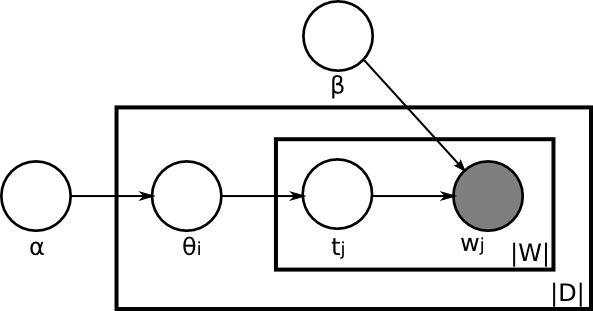
\includegraphics[width=6.5cm, height=3.2cm]{Latent_Dirichlet_allocation.png}\\
  \caption{Modelo gráfico LDA.} %\ref{joint:lda}.}
  \label{fig:lda}
\end{figure}

A implementação do LDA utilizada para estes experimentos está disponível no repositório \emph{online} de Alexandre Passos \cite{top-lda}, e o número de iterações para amostragem de tópicos e palavras foi fixado em 100. 


%O cálculo destas probabilidades também envolve integrais difíceis, ou mesmo impossíveis, de resolver analiticamente, o que implica no uso de técnicas de amostragem e aproximação. A amostragem de Gibbs, descrita superficialmente na seção \ref{subsection:bayes}, é uma alternativa para a geração de valores para variáveis aleatórias contidas no modelo \cite{gibbs-lingpipe}, sendo utilizada nos experimentos com LDA conduzidos neste projeto. 

%Quando um método de classificação é aplicado a um conjunto de documentos, a interpretação do resultado é imediata: cada documento estará associado a uma única classe. No caso do modelo de tópicos LDA, a interpretação do resultado é mais subjetiva. É preciso observar as palavras que se associam com maior probabilidade a cada tópico, buscando algum tipo de semelhança entre elas, para inferir seus significados. 


% o agrupamento de palavras como \emph{beef}, \emph{sauce} e \emph{cheese} em torno de um mesmo tópico indica o bom funcionamento do LDA%As palavras associadas a cada tópico siderando que as receitas pertencem à culinária tradicional dos Estados Unidos. O primeiro tópico pode ser interpretado como \textbf{Receitas com Carne}, pois associa ingredientes comumente consumidos  
%\textbf{Análise}

\subsection{L-LDA}

O L-LDA é uma variação do LDA em que se restringe o número de tópicos associados a cada documento. Ou seja, as distribuições fixadas para os tópicos de cada documento não necessariamente são sobre todos os tópicos \ensuremath{t \in T}. Além disso, os tópicos presentes em cada documento são identificados antes da execução do modelo, o que diminui a subjetividade envolvida na interpretação de seus significados após o processamento. 

Um bom exemplo para ilustrar a aplicação deste modelo envolve um \emph{blog}, em que cada \emph{post} é marcado com um conjunto específico de \emph{tags}. Se cada \emph{tag} é interpretada como um tópico, é possível informar ao L-LDA em que \emph{posts} cada uma delas está presente, processar os \emph{posts} com o modelo e saber, após o processamento, quais palavras se associam mais fortemente a cada \emph{tag}. Neste exemplo, existe um mapeamento direto entre os tópicos e as \emph{tags}, conduzindo a uma interpretação mais imediata do significado de cada agrupamento de palavras.

Experimentos com o L-LDA foram desenvolvidos ao longo deste projeto, associando cada tópico, por exemplo, a uma perspectiva a ser minerada. Após a execução do modelo, as palavras mais fortemente associadas a cada perspectiva ilustram como os assuntos discutidos são enfocados por elas. Quanto mais duas perspectivas se distanciam, mais diferentes são as palavras que se associam com destaque a cada uma delas.

O L-LDA foi discutido pela primeira vez em um artigo de Ramage et al. \cite{llda}, aplicado ao problema de atribuição de crédito em páginas do \emph{site del.icio.us}, marcadas com múltiplas \emph{tags}. O artigo parte da hipótese de que, embora um documento possa estar marcado com várias \emph{tags} diferentes, nem sempre elas se aplicam igualmente a todas as palavras nele contidas. A ideia da atribuição de crédito, portanto, consiste em associar cada palavra do documento às \emph{tags} mais apropriadas e vice-versa. 

%Uma aplicação de L-LDA, sugerida neste artigo e bastante empregada neste projeto, envolve, após a associação de palavras a tópicos (neste caso, \emph{tags}), a extração de trechos do documento que as contenham. Isto conduz a uma compreensão melhor de como o conteúdo se associa aos tópicos separadamente. 

A implementação de L-LDA utilizada neste projeto também está disponível no repositório \emph{online} de Alexandre Passos \cite{top-llda}. O número de iterações para amostragem de tópicos e palavras, em todos os experimentos, foi fixado em 100.
% do envolvendo uma ou mais palavras associadas a uma \emph{tag} particular. 
%O resultado de um método de classificação consiste em associar cada documento de um conjunto Diferentemente de métodos de classificação, cujo resultado pode ser interpretado de forma obj

%Assim como discutido na seção \ref{subsection:bayes}, 
% tópicos é fixada multinomial  \ensure\ensuremath{d} se associa a tópicos \ensuremath{t \in T} com probabilidades diferentes, o que é determinado pela escolha de uma distribuição de probabilidade sobre os tópicos. Em seguida, cada tópico é tratado como uma distribuição sobre palavras e cada palavra \ensuremath{w_i} de \ensuremath{d} se associa a eles de acordo com estas distribuições. A probabilidade da \ensuremath{i}-ésima palavra de \ensuremath{d} pode ser calculada como 

%P(wi) = sum P(wi | ti = j) P(ti = j), j de 1 a T. 

%onde ti é uma variável latente - ou seja, cujo valor não é observável, mas sim inferido - referente a um tópico, P(wi | ti = j) é a probabilidade de wi se associar ao tópico j e P(ti = j) é a probabilidade de se obter o tópico j na distribuição fixada para o documento \ensuremath{d} \cite{pnas}.

 %\textbf{Falar das receitas.}
%\textbf{Falar do uso de Gibbs Sampling para inferência}


%\subsection{L-LDA}



%Como o cenário de classificação envolve documentos de teste, cujas classes não são informadas ao classificador, uma saída para utilizar adequada deve-se inicialmente amostrar uma classe para cada % o cálculo desses valores se torna bastante complexo. É necessário, portanto, utilizar alguma técnica de amostragem para estimá-los. Para este projeto, o método escolhido foi o \textbf{Gibbs Sampling}, por ser simples de implementar e obter boas estimativas em um curto espaço de tempo. A técnica será apresentada brevemente nesta seção

%Não é possível obter os valores de \ensuremath{\phi} 
%A fim de se buscar estimativas para o conjunto de parâmetros que melhor se adaptem a \ensuremath{D}, Os valores de \ensuremath{\phi}, entretanto, não são usados diretamente na classificação. Em vez disso, %gera-se o documento baseando-se em seus hiperparâmetros e em informações extraídas do corpus, obtendo-se estimativas

%O gibbs sampling só é necessário quando você
%quer calcular os parâmetros P(tk|c) e P(c) usando, além dos documentos
%rotulados, documentos não rotulados. O fato de de repente o modelo
%virar um mixture model cria problemas de não-identificabilidade, e as
%somas e produtos que entram nas integrais complicam as coisas
%bastante.

%Esses valores podem ser estimados para documentos de \ensuremath{D''} de acordo com algum método de amostragem. Para esse projeto, o método escolhido foi o \textbf{Gibbs Sampling}, pe


%as equações \ref{classe2} e \ref{palavra} \cite{gibbs-lingpipe}. Antes de tudo, entretanto,  Por questões de escopo, suas derivações não serão apresentadas nessa monografia. 



%\begin{equation}
%\label{palavra}
%\ensuremath{P(w_t | c_j ; \theta') \eq \frac{1 + \sum_{i = 1}^{|D'|}z_{ij}N(w_t, d_i)}{\sum_{s = 1}^{|V|}\sum_{i = 1}^{|D'|}z_{ij}N(w_s, d_i)}}
%\end{equation}

%onde \ensuremath{z_{ij}} é dado pela classe \ensuremath{y_i} de \ensuremath{d_i}: 1 quando \ensuremath{y_i = c_j} e 0 em caso contrário. \ensuremath{N(w_t, d_i) é o número de vezes que a palavra \ensuremath{w_t} ocorre em \ensuremath{d_i}. A esse valor, dá-se o nome de \textbf{contagem} da palavra \ensuremath{w_i} em \ensuremath{d_i}, informação muito utilizada nos métodos de classificação de documentos por perspectiva. O Capítulo \ref{chap3}, inclusive, é totalmente dedicado à discussão do uso dessa informação para essa tarefa. A probabilidade de se obter uma classe \ensuremath{c_j}, por sua vez, é dada por%where N(wt , di ) is the count of the number of times word wt occurs in document di
%and where zij is given by the class label: 1 when yi = cj and otherwise 0.



%Para a classificação de documentos ser bem-sucedida, os valores de \ensuremath{\phi} devem modelar \ensuremath{D} da melhor forma possível. Isso significa que não basta amostrá-los de acordo com os hiperparâmetros \ensuremath{\{\alpha, \beta, \gamma_1, ..., \gamma_|D|\}} para obter boas estimativas para os dois termos no numerador de \ref{teorema-bayes}. É preciso estimá-los de acordo com informações extraídas dos próprios documentos. % dessa equação. e  Além disso, assume-se, no modelo Naïve Bayes, que as palavras dos documentos são condicionalmente independentes, de modo que a equação \ref{teorema-bayes} pode ser reescrita como

%O modelo Naïve Bayes é composto de um conjunto de parâmetros \ensuremath{\theta}, conforme discutido na seção \ref{subsection:naive}. Para identificar a classe \ensuremath{y_i} de um documento \ensuremath{d_i \in D''}, é preciso estimar inicialmente valores para esses parâmetros, gerando um novo conjunto \ensuremath{\theta'}. Embora seja possível considerar apenas o conjunto de treinamento 



%Essas estimativas devem maximizar \ensuremath{P(\theta | D')} ou \ensuremath{P(\theta | D)}. Pelo Teorema de Bayes, tem-se que, no primeiro caso, \ensuremath{P(\theta | D') \prop P(D' | \theta)P(\theta)}. Para se maximizar essa relação, deve-se resolver um sistema de derivadas parciais do \ensuremath{log(P(\theta | D')} utilizando-se uma técnica denominada Maximum a Posteriori (MAP) \cite{nigam}, tópico que não será abordado nessa monografia. É suficiente saber que essa maximização conduz às expressões \ref{palavra} e \ref{classe2}, muito importantes para a compreensão dos próximos capítulos\footnote{Essas expressões podem variar um pouco, a depender do método utilizado para derivá-las. As versões apresentadas aqui foram retiradas da dissertação de Kamal Nigam \cite{nigam}.}. A probabilidade de se obter uma palavra \ensuremath{w_t \in V}, fixada uma classe \ensuremath{c_j}, é dada por



%O segundo caso é análogo.}



%O processo de maximização, em ambos os casos, é relativamente complexo, fugindo ao escopo dessa monografia. Ele conduz, entretanto, a expressões bastante simples matematicamente, utilizadas na implementação dos classificadores%obtidas, entretanto, são bastante simples matematicamente % Basicamente, elas são razões entre % baseiam exclusivamente no número de vezes que cada palavra ocorre em um documento ou em uma classe %relacionam o número de ocorrências de cada palavra ocorre em um documento ou em uma classe% utilizadas efetivamente pelos classificadorsentretanto, são  %O primeiro caso é mais simples, pois envolve apenas documentos para os quais já se conhecem as classes. % Por este motivo, ele será discutido inicialmente.% O segundo caso requer mais informações, sendo discutido % \ensuremath{\theta'}% que maximizem \ensuremath{arg max_j P(y_i = c_j | d_i ; \theta')}. Aplicando-se o Teorema de Bayes, tem-se que
 
                                                 %This is the value of θ that is most probable given the evidence of the training data and a prior.


%\begin{equation}
%\label{palavra}
%\ensuremath{P(w_t | c_j ; \theta') \eq \frac{1 + \sum_{i = 1}^{|D'|}z_{ij}N(w_t, d_i)}{\sum_{s = 1}^{|V|}\sum_{i = 1}^{|D'|}z_{ij}N(w_s, d_i)}}
%\end{equation}

%onde \ensuremath{z_{ij}} é dado pela classe \ensuremath{y_i} de \ensuremath{d_i}: 1 quando \ensuremath{y_i = c_j} e 0 em caso contrário. \ensuremath{N(w_t, d_i) é o número de vezes que a palavra \ensuremath{w_t} ocorre em \ensuremath{d_i}. A esse valor, dá-se o nome de \textbf{contagem} da palavra \ensuremath{w_i} em \ensuremath{d_i}, informação muito utilizada nos métodos de classificação de documentos por perspectiva. O Capítulo \ref{chap3}, inclusive, é totalmente dedicado à discussão do uso dessa informação para essa tarefa. A probabilidade de se obter uma classe \ensuremath{c_j}, por sua vez, é dada por%where N(wt , di ) is the count of the number of times word wt occurs in document di
%and where zij is given by the class label: 1 when yi = cj and otherwise 0.

%\begin{equation}
%\label{classe2}
%\ensuremath{P(c_j | \theta') \eq \frac{1 + \sum_{i = 1}^{|D'|}z_{ij}}{|C| + |D'|}}
%\end{equation}

%Não é possível aplicar as equações \ref{palavra} e \ref{classe2} diretamente no segundo caso, pois o classificador não sabe que classes correspondem aos documentos de \ensuremath{D''}. Para se obter boas estimativas para \ensuremath{\theta} nesse caso, uma saída é utilizar um método de amostragem, como \ensuremath{Gibbs Sampling}. %- e, consequentemen neste caso, conduzindo  % \ensuremath{\theta'} considerando todos os documentos de \ensuremath{D}, uma saída é utilizar um método de amostragem, como Gibbs Sampling. amostrar, inicialmente, a classe de cada \ensuremath{d \in D''}, considerando as distribuições de probabilidade \ref{theta_c} e \ref{classe} apresentadas na seção \ref{subsection:naive}. Neste momento, é interessante que a escolha de qualquer classe seja equiprovável, dado que não se sabe quantos documentos de \ensuremath{D''} efetivamente pertencem a cada uma delas. Com todos os documentos rotulados, é possível obter uma estimativa para \ensuremath{P(\theta | D)}, mas nada garante que ela seja a melhor possível. O que deve ser feito, neste caso, é reclassificar os documentos de \ensuremath{D''} diversas vezes, até que se estabilizem os valores estimados para \ensuremath{\theta} - ou seja, até que o modelo convirja. Esses valores configuram uma estimativa ótima para \ensuremath{\theta}. Para reclassificar os documentos de \ensuremath{D''}

%utilizar as equações \ref{palavra} e \ref{classe2}, trocando \ensuremath{D'} por \ensuremath{D}. O que se obtêm, entretanto, não são estimativas ideais para \ensuremath{w_t} e \ensuremath{c_j}, pois os parâ


%Entretanto, essa primeira classificação não é suficiente, pois os parâmetros obtidos não necessariamente maximizam \ensuremath{P(\theta | D)}. Para se obter os melhores parâmetros que modelam \ensuremath{D} % e utilizar esses valores para 


%Dizer que isso é preferível pois modela melhor.

 %  parte dos documentos contidos em \ensuremath{D} (\ensuremath{D''}). %o segundo caso, antes de resolver a maximização que conduz a equações análogas a \ref{palavra} e \ref{classe}, é preciso estimar valores iniciais  % tamb
%the highest posterior probability, arg maxj P(yi = cj |di ; θ)


% O objetivo inicial do classificador Naïve Bayes, portanto, é obter um \ensuremath{\theta} que maximize \ensuremath{P(\theta | D')} ou \ensuremath{P(\theta | D)}. No primeiro caso, tem-se, utilizando o Teorema de Bayes, que

%\begin{equation}
%\label{gerando-theta}
%\ensuremath{P(\theta | D') \eq \frac{P(D'|\theta)P(\theta)}{P(D')} 
%\end{equation}

%A maximização dessa equação é bastante complexa, fugindo completamente do escopo dessa monografia. A expressão obtida, entretanto, é fundamental para a compreensão dos próximos capítulos


 %conjunto de valores para eles que 




%dor de documentos a partir dele. Esta seção trata de documentos de texto em particular, por se tratarem do objeto básico de estudo deste projeto. 
%Sabe-se que, em um Naïve Bayes, assume-se que as as características em um documento são condicionalmente independentes, o que equivale a afirmar, por exemplo, que a presença de uma palavra em um documento de texto não é informativa sobre a presença de nenhuma outra. Apesar desta hipótese simplificar bastante a estrutura linguística de um texto, classificadores construídos a partir do modelo Naïve Bayes, denominados classificadores Naïve Bayes, reportam um bom desempenho em várias tarefas de classificação baseadas em palavras \cite{naive-at-forty} \cite{mccallum-naive}.

%Dados um documento \ensuremath{d} pertencente a um conjunto de documentos \ensuremath{D}, todas as palavras distintas de \ensuremath{D}, \ensuremath{F_1, ..., F_k}, uma variável aleatória \ensuremath{c}, que representa as possíveis classes de \ensuremath{d}, e um vetor \ensuremath{v_d}, em que cada posição corresponde a uma de suas \ensuremath{n} palavras, tem-se que
 

%conforme discutido anteriormente na seção \ref{subsection:naive}. Um classificador Naïve Bayes deve rotular o documento \ensuremath{d} com o valor de \ensuremath{c} que maximiza a equação \ref{eq2:bayes}. Como o denominador na equação \ref{eq2:bayes} é o mesmo para todas as classes, ele pode ser ignorado nestes cálculos.

%Normalmente, classificadores Naïve Bayes são utilizados de forma semi-supervisionada. Isto significa que eles são submetidos a uma etapa de treinamento, na qual aprendem as classes associadas a alguns documentos, e a uma etapa de classificação, na qual devem simular o processo gerador destes documentos e utilizar esta informação para classificar outros. Basicamente, as informações aprendidas na etapa de treinamento modelam as distribuições das palavras de \ensuremath{D} por classe, gerando parâmetros para as distribuições de probabilidade envolvidas na classificação de outros documentos. 


%O número de iterações para amostragem de tópicos e palavras, em todos os experimentos, foi fixado em 100.

% a amostragem da equação \ref{eq:bayes} foi fixado em 500.

% classificando outros                        Dado que tenho exemplos de texto de cada classe. O
%que posso inferir sobre o processo gerador destes textos


%                              e                  o classificador reporta
%o melhor desempenho em v ́rias tarefas de classifica ̧ ̃o. Este fenˆmeno  ́
%                        a                         ca

 
%\begin{algorithm}
%\ensuremath{z^{(0)}} \gets \ensuremath{\langle z_1^{(0)}, \ldots, z_k^{(0)}\rangle}
%\FOR{\ensuremath{t = 1} to \ensuremath{T} do}
 % \FOR{\ensuremath{i = 1} to \ensuremath{k} do}
 %   \ensuremath{z_i^{(t + 1)} ~ P(Z_i | z_1^{(t + 1)}, \ldots, z_{i - 1}^{(t + 1)}, z_{i + 1}^{(t)}, \ldots, z_k^{(t)})}
 % \ENDFOR
%\ENDFOR

%\end{algorithm}


%Além disso, você deveria começar a descrever o naive bayes falando que
%ele é um modelo generativo e que assume independência condicional das
%features dado as classes. Dizer que naive bayes aproxima P(vetor(d),c)
%como sendo P(c) Produtorio(P(di|c), o que é a mesma coisa que dizer
%que as palavras são condicionalmente independentes dado as classes,
%mostrar como vc faz pra usar isso pra classificar, usando P(c|d)  =
%P(c,d)/P(d), e que como P(d) independe da classe pode ser ignorado se
%você quer encontrar a melhor classe. Daí você deveria especificar de
%onde vêm essas probabilidades, colocando uma prior Beta(alpha, alpha)
%em P(c) e uma prior Dirichlet(alpha) em P(tk|c).

%Dado um conjunto de documentos \ensuremath{D} e um conjunto de classes \ensuremath{C}, o classificador Naïve Bayes estima, através da aplicação do Teorema de Bayes,  a probabilidade de cada \ensuremath{d \in D} ser de cada uma das classes \ensuremath{c \in C}. Com estas probabilidades calculadas, o classificador determina, para todo \ensuremath{d}, qual é a classe \emph{c} a que ele estará associado. Esta classe pode, por exemplo, ser aquela para a qual a probabilidade obtida foi simplesmente a mais alta \cite{durant-smith} \cite{naive-forty}.

%Este tipo de classificador parte da ideia de que as informações presentes em um documento, utilizadas na determinação de sua classe, são independentes entre si. No caso de um documento de texto, assume-se que a presença ou ausência de um termo - uma palavra ou uma sequência de palavras - é independente da presença ou ausência de qualquer outro. Definida esta hipótese, a probabilidade de que um documento \emph{d} seja de uma classe \emph{c} é tal que

%\begin{equation}
%\label{eq1}
%\ensuremath{P(c|d) \propto P(c)\prod_{k=1}^{t_d}P(t_k|c)}  
%\end{equation} 

%onde \ensuremath{P(t_k|c)} é a probabilidade condicional do termo \ensuremath{t_k}  ocorrer em um documento da classe \ensuremath{c},  \ensuremath{P(c)} é a probabilidade a priori de um documento qualquer pertencer à classe \ensuremath{c} e \ensuremath{t_d} é o número de termos em \emph{d} \cite{stanford-IRbook}.

%As probabilidades envolvidas na relação \ref{eq1} contêm integrais díficeis ou mesmo impossíveis de se calcular analiticamente. Para calcular \ensuremath{P(c|d)}, portanto, utiliza-se aproximações obtidas através de técnicas de amostragem. Uma destas técnicas, comum na literatura de Aprendizado de Máquina e empregada neste projeto, é a amostragem de Gibbs. Em uma iteração da amostragem, a técnica condiciona as probabilidades calculadas para um documento \ensuremath{k} às classificações obtidas para os \ensuremath{k - 1} documentos anteriores \cite{resnik-gibbs}. A técnica está descrita, de forma básica, no algoritmo \textbf{X (o algorithm2e.sty tá dando pau)}.
                             % The basic idea in Gibbs sampling is that, rather than probabilistically picking
%the next state all at once, you make a separate probabilistic choice for each of the k dimensions, where each
%choice depends on the other k − 1 dimensions.


%A hipótese de independência entre os termos, razão pela qual o Naïve Bayes tem este nome\footnote{Naïve é uma palavra de origem francesa que significa "ingênua"}, simplifica bastante a estrutura da informação contida nos documentos. Ainda assim, o classificador costuma apresentar boas performances em categorização de textos, sendo utilizado, por exemplo, como base metodológica para alguns filtros de \emph{spam} \cite{paul}. Para melhorar o desempenho do Naïve Bayes, é comum fixar um conjunto de documentos previamente classificados de forma correta e utilizar a informação sobre suas classes na determinação das classes de outros documentos. Ao conjunto de documentos previamente classificados, dá-se o nome de \textbf{conjunto de treinamento}; ao conjunto de documentos a serem classificados, \textbf{conjunto de teste}.

 %Através do uso de Amostragem de Gibbs, a cada iteração se obtém uma aproximação melhor O número de amostras coletadas envolvendo cada classe foi fixado em 500. 
 
 
%     We shall assume for the moment that the training data set is linearly separable in
%feature space, so that by definition there exists at least one choice of the parameters
%w and b such that a function of the form (7.1) satisfies y(xn ) > 0 for points having
%tn = +1 and y(xn ) < 0 for points having tn = −1, so that tn y(xn ) > 0 for all
%training data points.


%Suppose some given data points each belong to one of two classes, and the goal is to decide which class a new data point will be in. In the case of support vector machines, a data point is viewed as a p-dimensional vector (a list of p numbers), and we want to know whether we can separate such points with a p − 1-dimensional hyperplane. This is called a linear classifier. There are many hyperplanes that might classify the data. One reasonable choice as the best hyperplane is the one that represents the largest separation, or margin, between the two classes. So we choose the hyperplane so that the distance from it to the nearest data point on each side is maximized. If such a hyperplane exists, it is known as the maximum-margin hyperplane and the linear classifier it defines is known as a maximum margin classifier.

% cada documento do corpus é representado como um vetor \ensuremath{x} em um espaço euclidiano \ensuremath{\mathbb{R}^M}. Na etapa de treinamento, \ensuremath{N} documentos, com suas respectivas classes \ensuremath{c_0} ou \ensuremath{c_1}, são apresentadas ao classificador, que deve aprender uma função e a classificação envolve o aprendizado de uma função que corte este hiperplano, dividindo os pontos em duas classes distintas. 





\chapter{Classificação por perspectiva: revisão e discussão}
\label{chap3}

A classificação de documentos de acordo com suas perspectivas é um tópico de pesquisa relativamente novo. Ele foi proposto como subproblema da área de Mineração de Opinião em 2008, pelas pesquisadoras Bo Pang e Lillian Lee \cite{omsa}. De acordo com elas, esse subproblema se diferencia da classificação por opinião por não configurar as classes como pólos (\emph{positivo}, \emph{negativo} etc.). De fato, a classificação por perspectiva visa a separar os documentos de um corpus de acordo com pontos de vista diferentes, como \emph{pró-Israel} ou \emph{pró-Palestina}. Embora, em certo nível, isso também polarize o corpus, já que normalmente os pontos de vista são antagônicos, dividi-lo de acordo com suas perspectivas é uma tarefa mais subjetiva do que aquela envolvendo opiniões. Um bom exemplo da diferença entre um ponto de vista e uma opinião, no contexto dos trabalhos revisados e de acordo com a \emph{survey} de Pang e Lee, é o seguinte: \emph{'Matrix' é um filme excelente} (opinião sobre um objeto específico, mais pontual) e \emph{a paz mundial dificilmente será alcançada} (ponto de vista sobre um tema; algo que pode implicar em uma série de opiniões alinhadas com este pensamento). Apesar de ter sido proposto formalmente apenas em 2008, uma conferência importante para a área de Mineração de Opinião, a \emph{AAAI\footnote{\emph{Association for the Advancement of Artificial Intelligence}.} Conference}, lançou, na edição de 2010, uma seção específica para trabalhos nesta direção: \emph{Sentiment and Perspective}\footnote{www.aaai.org/Conferences/AAAI/2010/aaai10schedule.pdf}. Isso indica que o subproblema deve se fortalecer como área de pesquisa nos próximos anos.

A \emph{survey} de Pang e Lee, uma das principais referências para este projeto, elenca três trabalhos que fazem classificação por perspectiva, na seção em que discute o tema. Todos eles foram publicados entre os anos de 2004 e 2006. Assim como nessa \emph{survey}, esta monografia explora trabalhos recentes, publicados entre 2000 e 2010. A metodologia aplicada na busca por trabalhos a serem revisados pode ser resumida nos seguintes passos:

\begin{enumerate}
\item Consideração dos três trabalhos indicados na \emph{survey} de Pang e Lee;
\item Busca, no \emph{Google Scholar}, por trabalhos citados nesses artigos;
\item Busca, no \emph{Google Scholar}, por trabalhos que citam os artigos coletados nos itens anteriores;
\item Busca, na \emph{ACL Anthology}\footnote{A \emph{Association of Computational Linguistics}, \emph{ACL}, mantém o maior arquivo digital envolvendo trabalhos de Linguística Computacional, o que inclui Mineração de Opinião (http://aclweb.org/anthology-new/).} pelas palavras \emph{perspective}, \emph{viewpoint}, \emph{politics}, \emph{political}, \emph{ideology} e \emph{ideological}. Estas palavras foram escolhidas por (1) funcionarem como sinônimos nos artigos coletados anteriormente ou (2) pela relevância em suas temáticas, escritos por especialistas;
\item Busca nos \emph{sites} dos eventos \emph{EMNLP\footnote{\emph{Empirical Methods in Natural Language Processing Conference.}}, NAACL\footnote{\emph{North American Chapter of the Association for Computational Linguistics Conference.}}, AAAI\footnote{\emph{Association for the Advancement of Artificial Intelligence Conference.}}} e \emph{CoNNL\footnote{\emph{Computational Natural Language Learning Conference.}}}, realizados entre 2000 e 2010, pelas mesmas palavras do item anterior. Esses eventos foram selecionados pela relevância na área de Mineração de Opinião. 
\end{enumerate}

Nem todos os trabalhos coletados, de acordo com essa metodologia, tinham necessariamente a ver com classificação por perspectiva. Alguns, como a tese de Alice Oh, se propõem modelar computacionalmente o conceito de perspectiva \cite{alice-oh}; outros, como o artigo de Laver et al., se propõem a criar uma escala ideológica e comparar documentos de acordo com ela \cite{wordscores}.  Por este motivo, foi feita uma filtragem que resultou em onze trabalhos a serem revisados. Na seção \ref{freqs:revisao}, essa revisão é apresentada. Grande parte dos trabalhos considera, ainda que não exclusivamente, as contagens de palavras dos documentos na classificação. Além disso, o uso dessas características, ou de alguma variação (como presença/ausência de palavras), envolve uma computação muito simples e não depende de nenhuma língua em particular. Diante desses fatores, a seção \ref{freqs:experim} discute a relação entre a classificação baseada em contagens de palavras e o emprego delas por diferentes perspectivas. %Por fim, na seção \ref{freqs:conc}, apresentam-se conclusões sobre os conteúdos expostos nas seções \ref{freqs:revisao} e \ref{freqs:experim}. 

\section{Trabalhos Revisados}
\label{freqs:revisao}

Todos os trabalhos revisados nesta seção apresentam uma metodologia em comum: eles organizam um corpus de documentos, definem em que perspectivas ele se divide, eventualmente pré-processam os documentos e, em seguida, classificam-nos utilizando alguma técnica - na maioria dos casos, SVMs ou Naïve Bayes. Independentemente da forma de classificação, tem-se que elas sempre se baseiam em características dos documentos para determinar suas classes. 
Quase todos os trabalhos revisados nessa seção exploram, como características, (1) contagens de palavras, ausência/presença de palavras ou alguma variação delas. Boa parte deles não testa o uso de nenhuma outra característica; alguns trabalhos as comparam com outras, que normalmente são seu enfoque. Essas outras características são escolhidas de forma muito particular, variando de um trabalho para outro. Em vez de apenas considerarem ocorrências de palavras em textos, esses trabalhos exploram (2) suas relações sintáticas, suas semânticas e também valores associados à proximidade temática/semântica entre dois ou mais documentos. Dado que essas últimas características variam bastante, e considerando também a popularidade das primeiras, decidiu-se dividir a revisão dos trabalhos nas seguintes subseções: a subseção \ref{contagem} apresenta trabalhos que classificam documentos baseando-se exclusivamente em (1); a subseção \ref{sintaxe} apresenta trabalhos que exploram (2) na classificação, exclusivamente ou em conjunto com (1). É importante informar que alguns trabalhos da segunda subseção, por questões comparativas, também classificam documentos exclusivamente de acordo com (1) - mas este não é o foco deles.  Por fim, na subseção \ref{compara}, é apresentada uma pequena análise comparativa envolvendo os trabalhos revisados nas subseções anteriores.

\subsection{Trabalhos que exploram contagem/presença de palavras ou variações}
\label{contagem}

O trabalho de \textbf{Lin et al.} classifica artigos do \emph{site} Bitterlemons\footnote{http://bitterlemons.org/} como pró-Palestina ou pró-Israel \cite{lin-et-al2006}. Inicialmente, os documentos são representados como listas de palavras reduzidas a seus radicais. Isso significa, por exemplo, que as palavras \emph{political} e \emph{politics} são representadas através de um mesmo termo, o radical \emph{politic}. Os classificadores Naïve Bayes e SVM são então aplicados, explorando as contagens desses radicais em cada documento. A taxa de acerto obtida com o SVM variou entre 81.48\% e 97.24\%; com o Naïve Bayes, ela variou entre 84.85\% e 99.09\%. Essas variações advêm de diferentes divisões entre os conjuntos de treinamento e teste. Por fim, o trabalho de Lin et al. propõe o classificador \emph{Latent Sentence Perspective Model}, ou simplesmente LSPM. Ele consiste em uma variação do Naïve Bayes que, em vez de considerar documentos como listas de palavras, os representa como listas de senteças. A hipótese assumida por ele é a seguinte: nem todas as sentenças carregam um ponto de vista, de modo que o classificador, antes de definir a classe de um documento, deve selecionar quais delas carregam palavras relevantes. A taxa de acerto obtida com o LSPM variou entre  86.99\% e 94.93\%, também como consequência de diferentes divisões entre os conjuntos de treinamento e teste. Para essas divisões, as taxas de acerto obtidas com o Naïve Bayes foram de 84.85\% e 93.46\%. O SVM não foi comparado diretamente com o LSPM. Apesar do desempenho superior a do Naïve Bayes, nenhum outro trabalho revisado faz uso desse classificador. 

\textbf{Mullen e Malouf} propõem dois trabalhos que analisam um conjunto de \emph{posts} do fórum de discussão política Politics\footnote{http://politics.com}. No \textbf{primeiro trabalho}, eles tratam cada documento como a união de todos os \emph{posts} de um mesmo usuário \cite{aaai-politics}. Cada documento é representado como uma lista de palavras, e um Naïve Bayes é aplicado considerando suas contagens em cada documento. A taxa de acerto obtida, via validação cruzada de dez dobras, foi de 60.37\%. O tamanho do \emph{dataset} (apenas 185 documentos) e o uso parecido de palavras por ambas as ideologias foram apontados como alguns dos principais motivos para a obtenção desse resultado. Mullen e Malouf também sugerem que a presença de documentos menores, correspondentes a usuários do fórum que raramente postam, pode contribuir negativamente para o desempenho do Naïve Bayes. Uma última observação desse trabalho indica o que pode estar acontecendo: usuários liberais citam falas de usuários conservadores em 62.2\% de seus \emph{posts}; analogamente, conservadores citam liberais em 77.5\%  de seus \emph{posts}. A presença das perspectivas liberal e conservadora em um mesmo documento, com uma correspondendo às intenções do usuário e outra sendo citada, pode homogeneizar o uso de palavras no corpus, comprometendo a viabilidade da classificação.

%A ideia é que, como esses usuários participam muito pouco do fórum, as palavras em seus \emph{posts} não são suficientes para se consolidar uma perspectiva, tornando-os mais difíceis de se classificar. Restringindo a classificação a usuários que postaram no fórum pelo menos 20 vezes, a taxa de acerto obtida com o Naïve Bayes foi ligeiramente superior (61.38\%).  Embora o artigo não indique a proporção média entre essas citações e o restante dos documentos, é possível que elas estejam interferindo negativamente no aprendizado das perspectivas. 

%Os documentos devem ser classificados, portanto, como alinhados com uma dessas duas ideologias. , escrito por cidadãos comuns dos Estados Unidos \cite{aaai-politics} \cite{malouf-taking_sides}. Em ambos, apesar de admitirem a diversidade de posicionamentos contidos no fórum, os autores dividem os documentos em apenas duas perspectivas, por uma questão de simplicidade: liberal e conservadora.

Essa forma de interação entre os participantes do fórum é explorada pelo \textbf{segundo trabalho de Mullen e Malouf} \cite{malouf-taking_sides}, com o intuito de melhorar a classificação. Para isto, cria-se um grafo de co-citação em que cada vértice representa um participante e cada citação em uma fala a outra é indicada por uma aresta entre seus autores. Os participantes são agrupados de acordo com seus padrões de citação e, em seguida, as falas de cada grupo obtido são tratadas como um único documento. Aplica-se um Naïve Bayes a esta nova coleção de documentos, também explorando apenas suas contagens de palavras, e os resultados obtidos são propagados para todos os participantes de cada grupo. Essa metodologia atinge resultados significativamente melhores do que aqueles obtidos no trabalho anterior: para participantes com mais de 500 palavras de fala no fórum, a taxa de acerto relatada é de 73\%. É válido salientar que, muito provavelmente, o sucesso dessa técnica é consequência do fato de que usuários alinhados ideologicamente não se citam muito. Se, além de citar seus oponentes, eles também se citassem bastante, os padrões de citação seriam sempre muito parecidos, inviabilizando os agrupamentos adequados no grafo.

O trabalho de \textbf{Durant e Smith} constrói um corpus sobre os posicionamentos do ex-Presidente George W. Bush quanto à Guerra do Iraque \cite{durant-smith}. O objetivo desse trabalho é classificar \emph{posts} de diversos \emph{blogs} políticos de acordo com os pontos de vista pró Guerra do Iraque e anti Guerra do Iraque.  Os classificadores Naïve Bayes e SVM foram aplicados, considerando apenas a presença/ausência de palavras nos documentos. A taxa de acerto obtida com um SVM foi de 75.47\%. Com o Naïve Bayes, ela foi de 78.06\%. Os autores, em seguida, investigam se a seleção de apenas parte das palavras pode melhorar a classificação. Eles aplicam uma técnica denominada \emph{CfsSubsetEval}, disponível na ferramenta WEKA 3.4\footnote{http://www.cs.waikato.ac.nz/ml/weka/}, que busca um subconjunto de palavras que maximize a taxa de acerto obtida. As palavras devem ter alta correlação com as classes escolhidas, mas baixa correlação entre si. Aplicando os classificadores SVM e Naïve Bayes, e considerando apenas os subconjuntos selecionados pela técnica, as taxas de acerto obtidas foram de 87.66\% e 89.77\%, respectivamente. É válido ressaltar que a técnica \emph{CfsSubsetEval} pode trazer uma melhoria de desempenho significativa para \emph{datasets} escritos em qualquer língua.

O trabalho de \textbf{Hirst, Riabinin e Graham} constrói dois \emph{datasets}, um em inglês e outro em francês, que consistem de discursos de congressistas canadenses nas reuniões parlamentares \cite{hirst-et-al}. Além de classificar esses discursos como liberais ou conservadores, esse trabalho investiga se as classes correspondem de fato a ideologias diferentes ou, simplesmente, a expressões de ataque e defesa. Inicialmente, os autores analisam o \ensuremath{36^o} parlamento canadense, período em que um partido liberal estava com a maioria no poder. Excluindo apenas as palavras menos frequentes do corpus, e aplicando um SVM baseado apenas nas contagens de palavras dos documentos, as taxas de acerto obtidas foram de 83.8\% e 75.5\% para os corpora inglês e francês, respectivamente. Em seguida, os autores selecionaram o \ensuremath{39^o} Parlamento, período em que os partidos liberais eram oposição, para verificar o que de fato estava determinando a classificação. Treinando com documentos do \ensuremath{36^o} Parlamento e testando com aqueles do \ensuremath{39^o}, a classificação entre liberal e conservador é insatisfatória: as taxas de acerto foram de 44.9\% e 45.7\% para os corpora inglês e francês respectivamente. Treinando com o \ensuremath{39^o} e testando com o \ensuremath{36^o}, as taxas de acerto foram ainda piores: 36.8\% e 35.2\% para os corpora inglês e francês respectivamente. Diante disso, os autores concluem que que as ideologias liberal e conservadora não são exploradas adequadamente pelos discursos. Se o fossem, e considerando que elas não mudaram significativamente de um parlamento para o outro, estes últimos experimentos apresentariam resultados melhores. Eles indicam que os discursos envolvem muitas expressões de ataque e defesa, que mudam de partido conforme eles se alternam no poder. Por este motivo, os conjuntos de treinamento e teste apresentam padrões de ataque e defesa invertidos, implicando no mau desempenho da classificação. Esse trabalho alerta, portanto, para a definição adequada de que perspectivas estão contidas no corpus. Neste caso, em vez de liberal e conservadora, seria mais adequado utilizar pró-governo e anti-governo, ou situação e oposição. % fixam as palavras que ocorrem menos frequentemente nos corpora foram removidas, e um SVM foi aplicado.

O trabalho de \textbf{Klebanov, Beigman e Diermeier} avalia o desempenho dos classificadores Naïve Bayes e SVM, utilizando para isso características diferentes dos documentos. Para o Naïve Bayes, os autores comparam a escolha entre (1) presença/ausência de palavras e (2) contagens de palavras. Para o SVM, as comparações envolvem a escolha entre (1), (3) suas contagens normalizadas em relação ao documento (frequências) e (4) suas frequências ponderadas em relação aos outros documentos do corpus. É válido ressaltar que todas essas características são apenas variações de contagens de palavras. Os autores selecionaram quatro \emph{datasets} para comparar essas escolhas: o primeiro envolve debates sobre o aborto, dividido entre pró-escolha e pró-vida; o segundo consiste em artigos sobre a pena de morte, dividido entre pró pena de morte e anti pena de morte; o terceiro é composto de artigos sobre o conflito Israel-Palestina, escritos por convidados do \emph{site} Bitterlemons e estudados por Lin et al. \cite{lin-et-al2006}; o quarto também é composto de documentos desse \emph{site}, cada um escrito por um especialista diferente. Esses dois últimos, assim como no trabalho de Lin et al., são divididos entre pró-Palestina e pró-Israel.  No caso do Naïve Bayes, o uso de (1) se mostrou melhor em alguns \emph{datasets} e o de (2), em outros. A maior diferença de desempenho observada está relacionada com o corpus de pena de morte: com (1), a taxa de acerto obtida foi de 88\%; com (2), 93\%. Os autores indicam, diante disso, que essa escolha não é tão relevante para problemas de classificação por perspectiva. Quanto ao SVM, a escolha por (1) se mostrou superior ou equivalente às outras em todos os casos. A maior diferença de desempenho observada também está associada ao corpus de pena de morte: enquanto (1) conduz a uma taxa de acerto de 83\%, (3) resulta em 82\% e (4) em 73\%. Esse trabalho, assim como o de Durant e Smith \cite{durant-smith}, também investiga o uso de um subconjunto de palavras. Com o apoio do \emph{toolkit} WEKA, os autores selecionam subconjuntos pequenos, contendo entre 100 e 500 palavras, e indicam que a classificação dos \emph{datasets}, nestes casos, conserva seu desempenho. As taxas de acerto não aumentam, como no trabalho de Durant e Smith, mas também não diminuem.




%esses dois pontos de vista. Inicialmente, foi feita uma seleção de \emph{blogs} baseada no \emph{site The Moderate Voice}\footnote{http://themoderatevoice.com/}. Este \emph{site} elenca \emph{blogs} de esquerda, direita e moderados. Para esse trabalho, Durant e Smith exploraram apenas os \emph{blogs} de esquerda e direita. Em seguida, apenas os \emph{posts} que tratavam de Bush e da Guerra do Iraque foram separados para classificação. O material foi dividido por mês, devido à grande quantidade de \emph{posts}. Esse trabalho assume que \emph{blogs} de esquerda concentram o ponto de vista anti-Bush,  no que diz respeito a suas atitudes quanto à Guerra do Iraque. \emph{Blogs} de direita, por sua vez, concentram o ponto de vista pró-Bush. 


%O tutorial de Resnik e Hardisty sobre Naïve Bayes e LSPM sugere algumas equações para a implementação deste último \cite{resnik}, mas o próprio Resnik afirmou, em \emph{e-mail} endereçado à autora desta monografia, nunca ter conseguido replicar os resultados apresentados por Lin et al. \cite{email}. Aparentemente, portanto, o LSPM não é tão simples de implementar quanto o Naïve Bayes.  Lin et al. concluem, diante dessas comparações, que o LSPM apresenta desempenho superior ao do Naïve Bayes. N


%Os artigos foram extraídos do \emph{site} Bitterlemons\footnote{http://www.bitterlemons.org/} e estão divididos entre \emph{Palestinian} ou \emph{Israeli}. Os primeiros defendem pontos de vista pró-Palestina; os segundos, pró-Israel. Essa divisão é explorada mais à frente, de modo que o




\subsection{Trabalhos que exploram outras características dos documentos}
\label{sintaxe}

O trabalho de \textbf{Jiang e Argamon} constrói um corpus de documentos extraídos de \emph{blogs} sobre política escritos em inglês \cite{jiang-argamon}. Cada \emph{blog} é associado à perspectiva liberal ou conservadora, divisão explorada na classificação. Os documentos que constituem o corpus são apenas as páginas iniciais de cada um deles. Inicialmente, Jiang e Argamon aplicam um SVM às páginas, considerando apenas a presença/ausência de palavras nos documentos. A taxa de acerto obtida foi de 81.92\% e, considerando ambas as classes, tem-se que a precisão média foi de 81.76\%, a rechamada média foi de 81.93\% e a métrica F1 média foi de 81.79\%. Em seguida, as páginas foram reduzidas a suas sentenças subjetivas, através de uma seleção baseada no dicionário semântico \emph{General Inquirer}\footnote{http://www.wjh.harvard.edu/~inquirer/}. Para uma sentença ser escolhida, ela deveria conter pelo menos duas palavras categorizadas, segundo o dicionário, como pertencentes às categorias \emph{Dor}, \emph{Hostilidade}, \emph{Prazer} ou \emph{Virtude}, dentre outras. A taxa de acerto, neste cenário, subiu para 83.28\%. As precisão, rechamada e métrica F1 médias foram de, respectivamente, 83.26\%, 83.38\% e 83.24\%. Esse trabalho, por fim, busca extrair as expressões opinativas que mais se relacionam aos pontos de vista liberal e conservador, baseando-se nas sentenças subjetivas e em consultas ao dicionário \emph{General Inquirer}. O SVM é aplicado considerando a presença/ausência de palavras e, adicionalmente, a presença/ausência das expressões opinativas separadas para cada lado. A taxa de acerto neste cenário foi de 84.96\%. As precisão, rechamada e métrica F1 médias foram de, respectivamente, 83.24\%, 83.48\% e 83.27\%. As melhorias em relação ao uso exclusivo de ausência/presença de palavras, portanto, são pequenas. Além disso, essas metodologias não são facilmente adaptáveis a línguas que não dispõem de dicionários como o \emph{General Inquirer} \emph{online}.

%Apesar de melhorarem a taxa de acerto obtida inicialmente, essas metodologias são completamente dependentes da língua em que o corpus está escrito. Elas não são  % Os \emph{blogs} foram escolhidos de acordo com cinco catálogos \emph{online}: BlogCatalog, Blogorama, eTalkingHead, Campaigns and Elections e Best of the Web Blogs\footnote{http://blogcatalog.com, http://blogarama.com, http://etalkinghead.com, http://campaignsandelections.com e http://blogs.botw.org.}. A finalidade desse trabalho, portanto, é determinar o posicionamento político desses \emph{blogs}, considerando seu conteúdo mais imediato - suas páginas iniciais. %As metodologias empregadas são completamente dependentes da linguagem do corpus, por utilizarem dicionários desenvolvidos para o inglês. % português.

O trabalho de \textbf{Greene e Resnik} enfoca no estudo de um corpus sobre a pena de morte \cite{greene}. Esse corpus é posteriormente analisado no trabalho de Klebanov, Beigman e Diermeier \cite{klebanov}, apresentado na seção anterior. O objetivo do trabalho é classificá-lo de acordo com as perspectivas pró pena de morte e anti pena de morte, e a metodologia desenvolvida baseia-se na hipótese de que existe uma conexão entre a estrutura de uma sentença e seu ponto de vista. Neste sentido, os autores selecionam um conjunto de verbos relevantes no corpus, como \emph{kill} e \emph{murder}, e criam representações para todos os termos que se relacionam sintaticamente com eles. Essas representações consistem em tuplas que associam cada termo a seu papel sintático na frase. Esses papéis, por sua vez, podem ser \emph{sujeito}, \emph{objeto direto}, \emph{verbo transitivo}, dentre outros. A determinação desses papéis foi feita com o apoio do programa \emph{Stanford Parser}\footnote{http://nlp.stanford.edu/software/lex-parser.shtml}, adaptado à língua inglesa. Greene e Resnik então aplicam um SVM nos documentos reduzidos a essas representações, atingindo taxas de acerto de 82.09\% e 88.10\%, a depender da escolha de verbos. Em vez de uma lista de palavras, portanto, o SVM é aplicado a uma lista de tuplas. Para comparar sua metodologia, os autores aplicam o SVM a documentos representados como sequências de duas palavras (bigramas), todas reduzidas a seus radicais. Nesse caso, as taxas de acerto obtidas foram de 68.37\% e 71.96\%, também a depender da escolha dos verbos. Essa metodologia, portanto, traz uma melhoria muito significativa para a classificação desse corpus. Apesar disso, aplicando a mesma metodologia ao corpus sobre o conflito Israel-Palestina, estudado por Lin et al. \cite{lin-et-al2006}, Greene e Resnik não obtêm nenhuma melhoria significativa. Em alguns cenários, os resultados obtidos por Lin et al. são ligeiramente melhores; em outros, são aqueles apresentados por estes autores.

O trabalho de \textbf{Efron} constrói dois \emph{datasets}: um envolvendo artigos sobre a política dos Estados Unidos e outro composto de textos sobre artistas musicais \cite{efron}. O primeiro corpus é classificado de acordo com as perspectivas direita e esquerda e o segundo, de acordo com as orientações pró-alternativa ou pró-popular. Inicialmente, Efron classifica os dois corpora com um Naïve Bayes e um SVM. O autor não especifica se são utilizadas contagens de palavras ou alguma outra característica, mas afirma que os dois métodos se baseiam apenas nas palavras contidas nos textos. Com o Naïve Bayes, as taxas de acerto obtidas nestes corpora foram de, respectivamente, 64.71\% e 50.1\%. Para o primeiro corpus, a taxa de acerto obtida com um SVM foi de 72.96\%; quanto ao segundo, não foram realizados experimentos com o SVM por carência de recursos computacionais. A fim de melhorar as taxas de acerto,  Efron desenvolve uma classificação baseada em citações que não envolve contagens de palavras nem citações de um documento a outro, mas sim suas semelhanças temáticas. Na prática, Efron determina a perspectiva de cada documento de acordo com a probabilidade deles serem co-citados com  documentos fixados como referência para cada perspectiva. Essa probabilidade é estimada a partir dos números de documentos retornados pelo buscador AltaVista\footnote{http://altavista.com/} quando dois documentos são buscados, indicando co-citação entre eles. Essa metodologia de classificação, aplicada ao primeiro \emph{dataset}, resultou em uma taxa de acerto de 94.1\%. Quanto ao segundo, as taxas de acerto obtidas foram de 82.18\% e 88.84\%. No primeiro caso, todos os documentos foram considerados; no segundo, os menos co-citados foram descartados. Apesar de simples e aparentemente eficiente, essa metodologia apresenta uma séria limitação: se o corpus for composto de documentos pouco citados na Web, as classes podem ser estimadas erroneamente com uma alta frequência, não trazendo nenhuma melhoria significativa à classificação.

O trabalho de \textbf{Thomas, Pang e Lee} se propõe a determinar os pontos de vista de congressistas dos Estados Unidos quanto a novas leis \cite{get-out-the-vote}. O corpus é dividido entre as perspectivas suporte e oposição em relação a novas leis, e cada documento corresponde, a princípio, a uma fala de um congressista. Inicialmente, cada texto é classificado de forma isolada, através da aplicação de um SVM que considera a presença/ausência de palavras em cada um deles. As taxas de acerto obtidas foram de 66.05\% e 70.04\%, a depender do subconjunto de documentos classificado. Tratando cada documento como a concatenação de todas as falas de um mesmo congressista, as taxas obtidas com o SVM, considerando as mesmas características, foram de 70.00\% e 71.60\%. A fim de melhorar essas taxas de acerto, os autores comparam trechos de documentos e determinam valores positivos que representam o quanto eles concordam. Quando esses valores são menores do que um determinado \ensuremath{\theta} fixado, considera-se que não há indícios suficientes de que os documentos concordam; eles são, então, reduzidos a zero. Adicionalmente, os autores aproveitam os experimentos com o SVM para determinar o grau de preferência para classificar cada documento como suporte ou oposição. A classe escolhida para cada um deles deve ser aquela que favorece o seguinte cenário: (1) ela não deve, idealmente, ser a rejeitada pelo SVM e (2) documentos que concordam muito não devem ser associados a classes diferentes. As taxas de acerto obtidas, considerando cada documento como uma fala, variaram entre 70.81\% e 89.11\%, a depender do subconjunto classificado e do valor de \ensuremath{\theta}. Considerando cada documento como a concatenação de todas as falas de um mesmo congressista, as taxas de acerto obtidas variaram entre 71.28\% e 88.72\%, também a depender do subconjunto classificado e do valor de \ensuremath{\theta}. A determinação errônea de concordâncias entre documentos pode prejudicar significativamente a classificação. Além disso, de acordo com os próprios autores, a adoção dessa metodologia só traz benefícios quando há artigos difíceis de classificar individualmente.    

O trabalho de \textbf{Bansal, Cardie e Lee} propõe uma extensão ao trabalho de Thomas, Pang e Lee \cite{get-out-the-vote}, considerando também a \emph{discordância} entre documentos \cite{disagree}. A hipótese assumida em ambos os trabalhos é a mesma: se é difícil determinar a classe de um documento \emph{x}, mas sabe-se que ele concorda \emph{ou discorda} de um documento \emph{y}, fácil de classificar, a determinação da classe de \emph{x} também se torna mais fácil. O trabalho apresenta algumas estratégias para determinação dos valores de discordância e, em seguida, compara seus usos com a metodologia proposta por Thomas, Pang e Lee. Bansal, Cardie e Lee também lidam com valores negativos, associados à discordância. Na prática, é preciso mapear esses valores negativos em positivos, pois eles dificultam o problema de otimização envolvido na determinação das classes dos documentos. Esses mapeamentos são justamente o que diferencia uma estratégia de outra. Utilizando o mesmo \emph{dataset} analisado por Thomas, Pang e Lee, os autores deste trabalho obtêm resultados superiores ou equivalentes àqueles que consideram apenas a concordância entre documentos, para a maioria das estratégias testadas. As taxas de acerto, entretanto, não são informadas explicitamente neste trabalho, sendo representadas através de um gráfico comparativo.
%convote e disagree
%decidem considerar o quanto congressistas diferentes \emph{concordam}. Neste sentido, os autores 



\subsection{Análise comparativa}
\label{compara}

Os trabalhos revisados nesta seção propõem, em quase todos os casos, \emph{datasets} relacionados com questões políticas. Neste sentido, o trabalho de \textbf{Efron}, revisado na subseção \ref{sintaxe}, destaca-se por também abordar perspectivas sobre música (pró-alternativa e pró-popular) \cite{efron}. De fato, não é simples definir o que é um ponto de vista ou perspectiva, mas, considerando-se a discussão proposta na \emph{survey} de Pang e Lee \cite{omsa}, essas terminologias não abrangem apenas temáticas políticas - mesmo que seja mais fácil visualizá-las nesses contextos. Adicionalmente, Alice Oh, em seu trabalho sobre modelagem de perspectiva, aborda uma temática esportiva (jogos de \emph{baseball}) \cite{alice-oh}. Embora ela não lide com classificação, seu estudo envolve as perspectivas sobre os jogos, evidenciando que é possível explorar temáticas não-políticas. Seria interessante, portanto, ampliar os estudos de classificação por perspectiva para outros domínios sócio-culturais. Por fim, é importante escolher essas perspectivas com certo cuidado, de modo que elas correspondam efetivamente ao conteúdo do corpus. Neste sentido, o trabalho de \textbf{Hirst, Riabinin e Graham}, apresentado na subseção \ref{contagem}, apresenta uma boa discussão \cite{hirst-et-al}. 

Quanto à definição de perspectivas, todos os trabalhos revisados dividiram seus corpora em duas delas, associando cada uma a uma classe. Embora essas divisões sejam mais complexas do que o uso de pólos positivo e negativo, muito comum na classificação por opinião \cite{thumbs-up} \cite{peanut-gallery}, eles também contêm um  antagonismo, como no caso de \emph{liberal} e \emph{conservador}. Grande parte dos corpora estudados não foi pré-processada. Neste sentido, destaca-se o segundo trabalho de \textbf{Mullen e Malouf}, apresentado na subseção \ref{contagem} \cite{malouf-taking_sides}. Apesar da classificação em si ser simples, baseando-se apenas em contagens de palavras, a geração dos documentos envolve a formulação de um grafo e a análise de padrões de citação semelhantes. Esse foi o pré-processamento mais sofisticado, dentre os trabalhos revisados. No que diz respeito aos classificadores, foi observado que não há consenso quanto à escolha pelo Naïve Bayes ou por um SVM, principais técnicas abordadas. Aparentemente, o desempenho de ambos não difere muito; o que realmente apresenta um impacto na classificação é a escolha das características dos documentos, exploradas por algum dos classificadores. De todo modo, \textbf{Lin et al.} enfoca, em seu trabalho revisado na subseção \ref{contagem}, no desenvolvimento de um novo classificador, o LSPM \cite{lin-et-al2006}. Esse classificador apresenta um desempenho apenas um pouco superior ao do Naïve Bayes, além de não ter sido explorado por nenhum outro trabalho pesquisado. Por outro lado, os trabalhos de Efron, \textbf{Thomas, Pang e Lee} e \textbf{Bansal, Cardie e Lee} apresentam metodologias de classificação completamente diferentes do Naïve Bayes e dos SVMs, e obtêm melhorias significativas em seus resultados \cite{efron} \cite{get-out-the-vote} \cite{disagree}. Essas metodologias, entretanto, se fundamentam na exploração de um tipo de característica: a semelhança entre documentos. Elas não são genéricas como os SVMs, por exemplo. 

Os trabalhos revisados exploram características diferentes dos documentos e, até quando exploram as mesmas, podem escolher apenas um subconjunto delas ou investir no pré-processa mento dos documentos. Tudo isso contribui para a riqueza metodológica desses trabalhos, de modo que ainda não há consenso sobre qual é a melhor forma de classificar documentos de acordo com suas perspectivas. Aparentemente, a resposta para essa questão depende do cenário. Em alguns casos, a simples aplicação de um Naïve Bayes ou um SVM, baseando-se em contagens de palavras, já conduz a bons resultados. É o caso dos trabalhos de Lin et al., Hirst, Riabinin e Graham e \textbf{Klebanov, Beigman e Diermeier}, revisados na subseção \ref{contagem}, e de \textbf{Jiang e Argamon}, revisado na subseção \ref{sintaxe} \cite{lin-et-al2006} \cite{hirst-et-al} \cite{klebanov} \cite{jiang-argamon}. Em outros casos, é possível melhorar o desempenho utilizando \emph{ainda} apenas contagens de palavras. Nestes casos, a estratégia envolve mudar o pré-processamento dos documentos, como no segundo trabalho de Mullen e Malouf, ou escolher um subconjunto ótimo de palavras, como no trabalho de \textbf{Durant e Smith} \cite{malouf-taking_sides} \cite{durant-smith}. Quando essas mudanças não são suficientes, sugere-se a investigação do uso de outras características, como indicam os trabalhos de \textbf{Greene e Resnik}, Efron e Thomas, Pang e Lee, revisados na subseção \ref{sintaxe} \cite{greene} \cite{efron} \cite{get-out-the-vote}. O uso de outras características normalmente envolve a aplicação de \emph{softwares} de apoio e outros algoritmos, de modo que é melhor verificar antes se um Naïve Bayes ou SVM, baseado na simples contagem de palavras, já não resolve o problema. Além disso, a exploração de outras características nem sempre é facilmente adaptável a qualquer língua, como evidenciam os trabalhos de Greene e Resnik e Jiang e Argamon, e nem sempre apresentam uma melhoria significativa em relação a metodologias mais simples, como nesse último caso \cite{greene} \cite{jiang-argamon}.
 
\section{Discussão sobre o uso de palavras e a classificação baseada em suas contagens}
\label{freqs:experim}

Conforme discutido na seção anterior, contagens de palavras e algumas variações são as características \emph{mais exploradas} na classificação. Nem todos os trabalhos enfocam essas características, mas grande parte, no mínimo, compara suas metodologias com o uso de um Naïve Bayes ou SVM baseado nelas. Além de envolver apenas cálculos simples, o uso de contagens de palavras ou variações torna a classificação facilmente adaptável a \emph{datasets} escritos em qualquer língua. Trabalhos como os de \textbf{Greene e Resnik} e \textbf{Jiang e Argamon} \cite{greene} \cite{jiang-argamon}, revisados na subseção \ref{sintaxe}, evidenciam o quanto o uso de características sintáticas/semânticas depende da existência de \emph{softwares} ou dicionários de apoio, direcionados a uma língua específica. O uso de contagens de palavras, em particular, não depende de nada disso. Por fim, além de simples, o uso de contagens de palavras, ausência/presença de palavras ou variações muitas vezes conduz a bons resultados, como indicado na seção anterior. 

Diante desses fatores, essa seção explora a relação existente entre a classificação baseada em contagens de palavras e o emprego delas nos documentos. A ideia é ampliar o entendimento sobre o desempenho obtido nesse tipo de classificação, observando a forma como documentos, escritos sob pontos de vista diferentes, empregam palavras. A escolha por contagens de palavras, em vez de ausência/presença ou alguma variação, foi arbitrária, já que, diante dos trabalhos revisados, não há indícios de que uma das alternativas seja, em termos gerais, melhor do que outra. Por motivos semelhantes, o classificador utilizado nos experimentos dessa seção foi o Naïve Bayes. O trabalho de Ng e Jordan, por sua vez, indica o uso do Naïve Bayes quando os \emph{datasets} analisados são pequenos \cite{ng-jordan}. Como este é o caso de um dos corpora analisados, esse argumento reforça a escolha pelo Naïve Bayes. %Sendo assim, recomenda-se que, antes de explorar outras características, verifique-se o desempenho da classificação baseando-se exclusivamente nestas.


Se um classificador utiliza apenas as contagens de palavras dos documentos para identificar suas perspectivas, sua taxa de acerto é tão mais baixa quanto menos essas contagens mudam de uma perspectiva para outra. Em outras palavras, como a contagem de uma palavra é o número de vezes que ela ocorre, isso significa que, em corpus nos quais os documentos usam as palavras de forma muito parecida (ocorrências e contagens semelhantes), a classificação se torna mais difícil. Apesar dessa relação ser clara, não se conhece nenhum método para \emph{quantificá-la}.  O objetivo dessa seção, portanto, é \emph{ilustrá-la} através de alguns experimentos. Neste sentido, é feita uma comparação entre o uso de palavras em dois \emph{datasets}, classificados com um Naïve Bayes baseado em contagens de palavras. Para a análise do uso das palavras, será utilizado o modelo de tópicos L-LDA. 
%Como o seu entendimento amplia a compreensão dos resultados obtidos com esses classificadores, esta seção se detém a ilustrá-la através de alguns experimentos.
%APRESENTE OS DOIS DATASETS. JUSTIFIQUE PQ REFEZ EXPERIMENTOS OU PQ N ESCOLHEU O AAAI E SIM OUTRO. - OK 

O primeiro \emph{dataset} estudado é composto de artigos sobre o conflito Israel-Palestina\footnote{Esse corpus está disponível em http://sites.google.com/site/weihaolinatcmu/data}, estudado pela primeira vez por Lin et al. em trabalho revisado na seção anterior \cite{lin-et-al2006}. O segundo \emph{dataset} estudado provém de outro trabalho: o artigo de Thomas, Pang e Lee sobre debates de congressistas dos Estados Unidos\footnote{Esse corpus está disponível em http://www.cs.cornell.edu/home/llee/data/convote.html}, também apresentado na seção anterior \cite{get-out-the-vote}. O primeiro \emph{dataset} contém 594 artigos, divididos entre as perspectivas pró-Israel (297) e pró-Palestina (297); o segundo, 8126 falas em debates, dividos entre as perspectivas republicana (4044) e democrata (4046). Esse corpus também se divide entre as perspectivas suporte e oposição em relação a novas leis, explorada por Thomas, Pang e Lee. Nessa seção, a primeira divisão é adotada por questões didáticas. Assume-se que o público desse trabalho está mais familiarizado com posicionamentos republicanos ou democratas, amplamente divulgados nas mídias, do que com aqueles da segunda divisão. Isso fará diferença na compreensão da análise de palavras proposta nessa seção.

Inicialmente, considerando-se essas divisões dos \emph{datasets}, experimentos com o Naïve Bayes foram conduzidos. Não foi feito nenhum pré-processamento nos corpora, simplificando ainda mais a metodologia dessa classificação. Via validação cruzada de dez dobras, a taxa de acerto obtida para o primeiro corpus foi de 86.22\%; para o segundo, de 54.01\%. A investigação sobre como as palavras são empregadas nesses \emph{datasets}, divididas por perspectiva, amplia a compreensão sobre esses resultados.

%MOSTRE COMO OS MODELOS DE TÓPICOS SÃO USADOS NOS DOIS LADOS - ok

Para a investigação sobre o uso de palavras, foi feita uma aplicação do modelo L-LDA. Cada documento de ambos os \emph{datasets} foi associado a dois tópicos: um genérico, idêntico para todos eles, e outro referente à sua perspectiva. No primeiro corpus, essas perspectivas são pró-Israel ou pró-Palestina; no segundo, republicana ou democrata. Há portanto, em cada corpus, três tópicos diferentes. O uso de um tópico genérico associado a todos os documentos ajuda a identificar palavras muito comuns nos \emph{datasets}, independentemente de perspectiva. Essa é a diferença fundamental entre essa aplicação do L-LDA e a simples contagem de palavras em documentos, dividida entre duas perspectivas. Esse tipo de contagem não evidencia que palavras são \emph{mais escolhidas} em documentos escritos sob uma certa perspectiva e quais são \emph{muito utilizadas} por todos eles - informação que colabora para um maior entendimento das taxas de acerto supracitadas, obtidas com um Naïve Bayes. É válido ressaltar que, em alguns casos, essas palavras coincidem em dois ou mais tópicos. Se, dentre esses tópicos, o genérico não estiver presente, isso significa que ambas as perspectivas dão muito destaque a essa palavra. Se a coincidência envolver o tópico genérico, tem-se que a palavra, além de ser muito enfocada por pelo menos um dos outros tópicos, é também uma das mais comuns no corpus.

%MOSTRE AS PALAVRAS ELENCADAS E DISCUTA

As dez palavras mais frequentemente associadas a cada tópico, retirando-se artigos, conjunções, preposições, advérbios e pronomes pessoais, estão listadas nas Tabelas 3.1 e \ref{freqs:tab2}. Apesar de pequenas, essas listagens sugerem interpretações sobre como as palavras de cada corpus são exploradas por suas diferentes perspectivas. Essas interpretações, essencialmente  subjetivas, ajudam a entender o comportamento do classificador Naïve Bayes aplicado aos dois \emph{datasets}.%colaboram parsubjetiva de se ampliar a discussão sobre os resultados obtidos com o Naïve Bayes.

%provêem informações subjetivas sobre a linguagem empregada nos corpora.
%As palavras extraídas a partir da aplicação de um L-LDA  Ainda assim, essas informações 

%Para ilustrar a relação que existe entre as taxas de acerto do Naïve Bayes e o uso de palavras nesses corpora, a

%As análises feitas a partir dessas pequenas listagens são essencialmente subjetivas, sugerindo interpretações %sugerindo  Essa análise não pretende  % A partir disso, espera-se compreender melhor o 

\begin{table}[h]
\label{tab1}
\centering
\begin{tabular}{| l | p{10cm} | }
\hline
\textbf{Tópico} & \textbf{Palavras} \\ \hline
\textbf{Genérico} & israel, palestinian, israeli, palestinians, state, one, two, israelis, political, right \\ \hline
\textbf{Pró-Israel} & sharon, palestinian, arafat, peace, israeli, prime, bush, minister, american, process \\ \hline
\textbf{Pró-Palestina} & palestinian, israeli, sharon, peace, occupation, international, political, united, people, violence \\ \hline
\end{tabular}
\caption{As dez palavras mais frequentemente associadas aos tópicos pró-Israel, pró-Palestina e genérico, de acordo com um L-LDA.}
\end{table}


Considerando o primeiro corpus, as palavras associadas às perspectivas pró-Israel e pró-Palestina remetem de imediato ao conflito travado entre essas duas nações. Parte delas, como \emph{palestinian} e \emph{israeli}, são bastante mencionadas em ambas as perspectivas, ainda que com propósitos diferentes: %israelenses, 

\begin{quote}

\emph{"The recent \textbf{Israeli} government decision to begin building extensive walls
around \textbf{Palestinian} is just one more example of how \textbf{Israeli} Prime
Minister Ariel Sharon is unable to deal with \textbf{Israeli} problems save
through his narrow security vision."}

{\small Retirado de "Peace in peaces", de Ghassan Khatib (pró-Palestina) - 10/06/2002}
\end{quote}

\begin{quote}

\emph{"The first conclusion that the Israeli political and security
establishment should learn and internalize after 18 months of
\textbf{Palestinian} Intifada, concerns the intensity of \textbf{Palestinian} blind
terrorism and guerilla warfare against the State of Israel."}

{\small Retirado de "The lessons Israel should learn", de Meir Pa'il (pró-Israel) - 29/04/2002}
\end{quote}

%\emph{"Meanwhile, the Israeli army was still suffering in South Lebanon as a result of the dilemma that \textbf{Sharon} put them in."}

%{\small Retirado de "Sharon settles accounts", de Mamdouh Nofal (pró-Palestina) - 28/01/2002}

Outras palavras, como \emph{bush} e \emph{occupation}, foram mais enfatizadas, respectivamente, pelas perspectivas pró-Israel e pró-Palestina, constando em apenas uma listagem. Os trechos abaixo evidenciam a importância, no período em que os documentos desse corpus foram escritos (2001 - 2005), do Governo Bush para Israel e da criação de um Estado para a nação palestina:
 %\textbf{Falar das figuras e de como elas deixam isso tão claro.} 

%\textbf{FIGURAS} % Para compreender melhor o uso das palavras pelos diferentes pontos de vista do corpus, elas foram processadas pelo software wordle22 , resultando nas figuras 7.1, 7.2 e 7.3. O tamanho das palavras nas imagens corresponde ao quanto elas se associam a cada tópico23 .

%Falar das ênfases no próprio lado/lado oposto e mostrar tb as palavras genéricas.
%Os trechos abaixo, separados por perspectiva, ilustram dois contextos diferentes para o uso dessas palavras

%\begin{quote}
%\emph{"The recent \textbf{Israeli} government decision to begin building extensive walls
%around \textbf{Palestinian} is just one more example of how \textbf{Israeli} Prime
%Minister Ariel Sharon is unable to deal with \textbf{Israeli} problems save
%through his narrow security vision."} 

%{\small Retirado de \emph{"Peace in pieces"}, de Ghassan Khatib - 10/06/2002}
%\end{quote}

%\begin{quote}
%\emph{"The first conclusion that the Israeli political and security
%establishment should learn and internalize after 18 months of
%\textbf{Palestinian} Intifada, concerns the intensity of \textbf{Palestinian} blind
%terrorism and guerilla warfare against the State of Israel."} 

%{\small Retirado de }

%\end{quote}


\begin{quote}
\emph{"\textbf{Bush} and his advisers, who have been critical of Clinton's deep involvement
in a failed peace process ever since taking office, nevertheless
understood at the time that peace in the Middle East should be beyond
politics in America, and that the US could not permit itself to turn its
back on an Israeli leader who was determined to make peace."} 

{\small Retirado de "Barak was willing, and so were US Jews", de Yossi Alpher (pró-Israel) - 15/07/2002}
\end{quote}

\begin{quote}
\emph{"But just as we were close to a complete
package that would have ended the \textbf{occupation} and established a
Palestinian state, Barak permitted Ariel Sharon's provocative visit to
Al Aqsa mosque, and launched his "revenge" on Palestinians."} 

{\small Retirado de "Guarding our legitimacy", de Samir Abdullah (pró-Palestina) - 14/10/2002}
\end{quote}

Associadas ao tópico genérico, também estão as palavras \emph{palestinian} e \emph{israeli}, bastante exploradas pelas duas perspectivas. Isso reflete a importância que esses termos têm para o corpus como um todo. Palavras relacionadas mais genericamente ao conflito Israel-Palestina, como \emph{state} e \emph{political}, também aparecem na listagem. %, evidenciando indica que essas palavras         


                     % A imagem 7.3 dá certo destaque a Lula e José Serra, mas também enfatiza outros termos, como governo e brasil, relacionados mais genericamente ao tema geral dos artigos: a política brasileira.


%Essas análises, avaliadas à luz das altas taxas de acerto obtidas com o Naïve Bayes, sugerem que os autores desse primeiro corpus defendem seus pontos de vista veementemente. Como eles são antagônicos, isso se reflete em enfoques diferentes a determinados termos, %empregos diferentes de palavras. % tornando a forma como empregam as palavras  defendem suas perspectivas utilizando palavras de forma suficientemente diferentedestacando ideias diferentes.

\begin{table}[h]
\label{freqs:tab2}
\centering
\begin{tabular}{| l | p{10cm} | }
\hline
\textbf{Tópico} & \textbf{Palavras} \\ \hline
\textbf{Genérico} & mr., speaker, bill, all, time, people, today, gentleman, federal, support \\ \hline
\textbf{Democrata} & bill, security, legislation, states, chairman, country, act, billion, million, law \\ \hline
\textbf{Republicano} & act, chairman, security, states, bill, legislation, 11, support, 9, system \\ \hline
\end{tabular}
\caption{As dez palavras mais frequentemente associadas aos tópicos republicano, democrata e genérico, de acordo com um L-LDA.}
\end{table}

%Considerando o primeiro corpus, as palavras associadas às perspectivas pró-Israel e pró-Palestina remetem de imediato ao conflito travado entre essas duas nações. Parte delas, como \emph{palestinian} e \emph{israeli}, são bastante mencionadas em ambas as perspectivas, ainda que com \textbf{intensidades} diferentes. \textbf{Falar das figuras e de como elas deixam isso tão claro.} 

%Falar q blz, aparecem palavras diferentes e tb há proporções diferentes, mas oq dá pra notar no geral eh q os termos envolvem pouca polêmica, e são usados de forma parecida. Isso, e o fato da amostra ser pequena, sugere q os debatentes n defendem as perspectivas republicana e democrata de forma suficientemente clara pra q um Naïve Bayes classifique corretamente.

Considerando o segundo corpus, tem-se que parte das palavras associadas às perspectivas republicana e democrata, como \emph{bill}, \emph{legislation}, \emph{states} e \emph{act}, tem mais a ver com o processo legislativo em si do que com alguma delas. Isso sugere que os debatentes não focam seus discursos na defesa de ideias republicanas ou democratas. Além disso, algumas dessas palavras são, muitas vezes, empregadas com conotações semelhantes por democratas e republicanos. Um exemplo é a palavra \emph{security}, como pode ser observado nos trechos abaixo

\begin{quote}
\emph{"Mr. speaker, I wholeheartedly agree that if we want to cut down on illegal immigration, we must improve border \textbf{security}. Just 2 weeks ago, an astute crane operator at the port of Los Angeles discovered 32 Chinese stowaways in a container that had just been unloaded from a Panamanian freighter."} 

{\small Retirado de discurso de Jane Harman, democrata - 09/02/2005 }

\end{quote}

\begin{quote}
\emph{"The fence remains incomplete and is an opportunity for aliens to cross the border illegally. This incomplete fence allows border \textbf{security} gaps to remain open.  We must close these gaps because they remain a threat to our national \textbf{security}."}

{\small Retirado de discurso de John Boozman, republicano - 02/10/2005}

\end{quote}

Duas palavras listadas apenas para a perspectiva republicana, \emph{11} e \emph{9}, podem sugerir um maior enfoque no episódio 11 de Setembro e seus desdobramentos. A palavra \emph{billion}, listada apenas para a perspectiva democrata, é muitas vezes utilizada para discutir gastos públicos, o que pode indicar um destaque maior para esse assunto

\begin{quote}
\emph{We know that all but one of the \textbf{9}/\textbf{11} hijackers acquired some type of U.S. identification documents. In fact, the 19 hijackers had 63 driver 's licenses among them.}

{\small Retirado de discurso de John Sullivan, republicano - 09/02/2005} 
\end{quote}

\begin{quote}
\emph{The Pomeroy bill would cost the treasury \$72 \textbf{billion} over 10 years, compared with the \$290 \textbf{billion} price tag of a full repeal through 2015, according to the joint committee on taxation.}

{\small Retirado de discurso de Earl Pomeroy, democrata - 12/04/2005}
\end{quote}


As palavras associadas ao tópico genérico, assim como aquelas associadas às perspectivas republicana e democrata, também têm mais a ver com o processo legislativo e a estrutura dos debates do que com posicionamentos políticos. Alguns exemplos são \emph{bill}, \emph{mr.}, \emph{speaker} e \emph{gentleman}. Isso reforça a ideia, apresentada por \textbf{Hirst, Riabinin e Graham} em trabalho revisado na seção anterior \cite{hirst-et-al}, de que a divisão entre as perspectivas republicana e democrata não é muito adequada para este corpus. De todo modo, uma divisão inadequada não necessariamente implica em mau desempenho: em uma classificação, esses autores obtiveram, utilizando uma divisão inadequada de corpus, uma taxa de acerto de 83.8\% \cite{hirst-et-al}. É válido ressaltar que eles utilizam \emph{apenas} contagens de palavras e exploram um \emph{dataset} muito semelhante a este: debates entre congressistas do Canadá. 

As Tabelas 3.1 e \ref{freqs:tab2} sugerem que os republicanos e democratas estudados no segundo corpus se expressam de forma mais parecida do que os autores do primeiro corpus. Este é o ponto que, de fato, pode contribuir negativamente para a classificação. Talvez isso advenha do fato de que seus discursos fazem parte de debates, o que pode concentrar as discussões em torno de um conjunto muito específico de termos. No primeiro corpus, os autores não escreveram seus artigos como resposta direta a outros, o que pode colaborar para que eles se expressem de forma mais autêntica e veemente, focando seus textos na apresentação de seus pontos de vista. A aplicação do L-LDA, associando cada tópico a uma perspectiva diferente, se mostrou válida, evidenciando uma certa homogeneização no uso de palavras no segundo corpus, quando comparado com o primeiro.
  %Associadas ao tópico genérico, há palavras referentes ao processo legislativo e aos debates, como \emph{bill}, \emph{mr.}, \emph{speaker} e \emph{gentleman}. Essas são as palavras mais comuns em todo o corpus - e, como pode ser observado, elas se assemelham às palavras elencadas para as perspectivas. Não apenas porque algumas delas, como blablala, estão listadas para os três tópicos, mas especialmente porque grande parte delas não evidencia um viés republicano ou democrata.%  Essa característica também é observada nas palavras listadas para as duas perspectivas, o que sugere a dificuldade de se identificar as perspectivas republicana ou democrática nos documentos desse segundo corpus. %  estão as palavras \emph{palestinian} e \emph{israeli}, bastante exploradas pelas duas perspectivas. Isso reflete a importância que esses termos têm para o corpus como um todo. Palavras relacionadas mais genericamente ao conflito Israel-Palestina, como \emph{state} e \emph{political}, também aparecem na listagem. 


%As taxas de acerto obtidas com um Naïve Bayes nesse segundo corpus foram baixas. % Ainda que as perspectivas republicana e democrata enfatizem palavras diferentes, conforme pode ser observado na Tabela \ref{freqs:tab2}, as listagens sugerem que elas empregam mais palavras em comum, no decorrer dos debates, do que os artigos  

As palavras das Tabelas 3.1 e \ref{freqs:tab2} foram representadas graficamente com o apoio do \emph{software} wordle\footnote{http://wordle.net/}. Apesar de se associarem aos tópicos com frequências distintas, o \emph{software} não foi sensível o suficiente para capturar essas diferenças. Por este motivo, essas imagens não constam nessa monografia.


É válido ressaltar que, a depender do \emph{dataset}, outras questões podem colaborar para um mau desempenho na classificação. Um conjunto de documentos com poucos exemplares, ou contendo poucas palavras, é um cenário onde a aplicação do Naïve Bayes pode não funcionar bem. Entretanto, esse não parece ser o caso dos corpora analisados nessa seção. De todo modo, quando não se obtém uma boa taxa de acerto com um classificador baseado em contagens de palavras, a investigação subjetiva de como cada perspectiva faz uso delas pode ajudar na compreensão do fenômeno. O tópico genérico, por sua vez, concentra as palavras mais comuns em todo o corpus. Se elas são muito semelhantes às palavras elencadas para cada perspectiva, isso também pode indicar uma certa homogeneização no uso das palavras. Nesses casos, é preciso buscar características dos documentos que os diferenciem melhor. %Apesar de não se quantificar a relação entre o uso de palavras no segundo corpus  sua classificação,  %A depender das conclusões retiradas, pode-se pensar em outras metodologias para a classificação dos documentos de acordo com suas perspectivas.


\chapter{Estudo de caso: Perspectivas sobre o governo brasileiro}
\label{estudo}
%Onde se motiva o estudo das eleições e fala pq tratará de colunas de jornalistas de notoriedade nacional. TUDO NESTE CAPÍTULO PRECISA SER BEM DIDÁTICO. FALAR DA FOLHA DILMAFACTSBYFOLHA

%mtos trabalhos de mineração de perspectiva tratam de discussão política. aproveitando o fato de que em 2010 se realizam as primeiras eleições para presidente realmente acompanhadas pela Internet, a gente decidiu fazer um estudo de caso neste assunto. Há outras pessoas pensando em coisas parecidas, como a galera do eleitorando, q criou o serviço pra fazer identificação de opinião em tweets. mas oq estamos propondo é fazer um estudo de análise das perspectivas contidas em blogs e colunas de jornalistas de notoriedade nacional, por eles serem muito lidos e contribuírem para a formação de opinião de seus leitores sobre o governo brasileiro, oq tem tudo a ver com a hora da urna. Mostre depois a estrutura da parades. fale de outros corpus e eleitorando

%Por ser um ano eleitoral, a

Muitos dos trabalhos revisados neste projeto analisam documentos que tratam de política. Em particular, boa parte deles estuda textos relacionados a governos federais - quer sejam discussões entre os próprios governantes, como nos estudos de \textbf{Thomas, Pang e Lee} \cite{get-out-the-vote} ou \textbf{Hirst, Riabinin e Graham} \cite{hirst-et-al}, quer sejam artigos escritos por cidadãos ou especialistas, como nos artigos de \textbf{Mullen e Malouf}\footnote{Todos os trabalhos mencionados nesta sentença foram revisados no Capítulo \ref{chap3}.} \cite{aaai-politics} \cite{malouf-taking_sides}. Considerando essa tendência, e o fato de que 2010 é ano de eleições para presidente no Brasil, decidiu-se realizar um estudo de caso que aproveita a abundância de artigos, disponíveis na \emph{Web}, sobre o governo Lula e da sucessão presidencial. A ideia é construir um corpus com alguns desses documentos e investigar suas perspectivas automaticamente, classificando-os de acordo com seus posicionamentos e analisando, de forma subjetiva, as palavras por eles enfocadas. É válido ressaltar que não foi encontrado nenhum outro trabalho, em português, que classifique documentos de acordo com seus pontos de vista.

%Os artigos escolhidos para este estudo foram extraídos de colunas, \emph{blogs} e \emph{sites} políticos mantidos por jornalistas de notoriedade nacional. A coleta de artigos contidos em \emph{blogs} escritos por cidadãos comuns também foi cogitada - entretanto, como eles são pouco conhecidos, comentados e divulgados, essa opção exigiria um esforço de análise manual dos \emph{posts} que foge ao escopo deste projeto. Além disso, uma vantagem em focar o estudo em material publicado por jornalistas conhecidos é poder correlacionar, posteriormente, os resultados obtidos a investigações sobre a formação de opinião na mídia brasileira \emph{online} - tanto na alternativa quanto na tradicional. A seleção dos veículos para este estudo de caso resultou do consenso entre a autora desta monografia e dois jornalistas \textbf{COMO CITÁ-LOS, DIZER SEUS NOMES?}. O critério básico para as escolhas foi a defesa clara de um ponto de vista sobre o governo Lula e/ou a sucessão presidencial de 2010. 

As próximas seções deste capítulo se estruturam da seguinte forma: na seção \ref{estudo:sec1}, a construção do corpus é apresentada - desde a seleção dos veículos até a definição dos pontos de vista explorados; na seção \ref{estudo:sec2}, experimentos com um classificador Naïve Bayes são conduzidos para, assim como em outros trabalhos revisados neste projeto, se classificar artigos de acordo com suas perspectivas; na seção \ref{estudo:sec3}, o modelo de tópicos L-LDA é aplicado ao corpus, evidenciando o uso de palavras por artigos com posicionamentos diferentes. 

% posicionamentos é analisada  
%Por serem muito lidos, e defenderem perspectivas claras nos textos que publicam, estes jornalistas têm o poder de influenciar muitos eleitores brasileiros. %análises  % mas requereria muito mais esforço de análise do que o uso exclusivo de documentos  %Lula é minha anta Dois jornalistas

\section{Construindo um corpus para estudo}
\label{estudo:sec1}

%O corpus deste estudo é composto de artigos escritos para colunas de jornais e revistas ou para \emph{sites} sobre política. São textos de caráter eminentemente opinativo, que diferem de notícias tanto pela finalidade - \textbf{blibli} - quanto pela linguagem - \textbf{blabla}. 

Os artigos escolhidos para este estudo foram extraídos de colunas, \emph{blogs} e \emph{sites} políticos mantidos por jornalistas de notoriedade nacional. A coleta de \emph{posts} de \emph{blogs} escritos por cidadãos comuns também foi cogitada - entretanto, como eles são pouco conhecidos, comentados e divulgados, essa opção exigiria um esforço de análise manual dos \emph{posts} que foge ao escopo deste projeto. Além disso, uma vantagem em focar o estudo em material publicado por jornalistas conhecidos é poder correlacionar, posteriormente, os resultados obtidos a investigações sobre a formação de opinião na mídia brasileira \emph{online} - tanto na alternativa quanto na tradicional. 

A seleção dos veículos para este estudo de caso resultou do consenso entre a autora desta monografia e os jornalistas Lucas Cunha Almeida e Andrea Duarte Bessa\footnote{Lucas Cunha, atualmente, é repórter do jornal baiano A Tarde; Andrea Bessa é gerente de comunicações da empresa Cetrel.}. O critério básico para as escolhas foi a defesa clara de um ponto de vista sobre o governo Lula e/ou a sucessão presidencial de 2010. Assim como em outros artigos revisados nesta monografia, que dividem os corpora analisados em dois lados antagônicos, assume-se que os artigos do \emph{dataset} desse estudo de caso dividem-se entre pró-situação e pró-oposição. Neste sentido, há autores que apóiam candidatos de ambos os lados, muitas vezes criticando o governo Lula e suas personalidades. Os trechos de \emph{posts} apresentados nessa seção reforçam a ideia de que essa divisão é adequada. O lado pró-situação é composto de artigos veiculados em:


%EXPLICAR Q POR SIMPLICIDADE E PQ QUASE TUDO ESTUDADO É ASSIM, DIVIDIU-SE AS PERSPECTIVAS A SEREM IDENTIF. AUTOM. EM PRÓ E ANTI GOVERNO
\begin{enumerate}

\item \textbf{Luis Nassif Online}\footnote{http://www.advivo.com.br/luisnassif/} Este é o \emph{blog} do jornalista Luis Nassif, premiado como Melhor Blog de Política pelo iBest 2008\footnote{http://idgnow.uol.com.br/internet/2008/05/21/ibest-2008-anuncia-vencedores/}. Nassif, que já trabalhou na TV Cultura e Rede Bandeirantes, mantém o \emph{blog} há cinco anos, enfocando principalmente assuntos relativos à política brasileira. Artigos do \emph{blog} são frequentemente citados, de forma positiva, em veículos de campanha pró-situação, como os \emph{sites} Blog da Dilma\footnote{http://dilma13.blogspot.com/} e Os Amigos do Presidente Lula\footnote{http://osamigosdopresidentelula.blogspot.com/}. De fato, o Luis Nassif Online adota um posicionamento pró-situação, como comprovam os trechos a seguir:

\begin{quote}
\emph{"Desde o ano passado, estava claro [sic] a falta de competitividade de José Serra, seja por não ter feito um governo brilhante em São Paulo, por não representar o novo e por não conseguir desenvolver um discurso próprio."}

{\small Retirado de \emph{"Em Minas, a mãe de todas as batalhas"} - 02/09/2010} 
\end{quote}

\begin{quote}

\emph{"Na entrevista, Bonner se limitou a perguntar da dependência de Dilma em relação à Lula [...] A consequência foi Dilma rebatendo com facilidade cada bobagem dita, reforçando o discurso social, mas sem avançar em uma proposta sequer de programa, explicando a lógica das alianças políticas. E William Bonner interrompendo-a a toda hora, impedindo sequer uma resposta completa. Algo tão desastrado e mal educado que obrigou Fátima Bernardes, do alto de sua elegância, a calá-lo com um sinal, para que parasse de ser inconveniente."}

{ \small Retirado de \emph{"O dia em que William Bonner escorregou"} - 10/08/2010}

\end{quote}

%Além de conter artigos escritos pelo próprio Luis Nassif, o \emph{blog} também publica textos de outros autores - alinhados, evidentemente, com os pontos de vista do jornalista. 

Como o veículo possui muito conteúdo, foram considerados apenas os artigos da categoria "Eleições".  

\item \textbf{Conversa Afiada}\footnote{http://www.conversaafiada.com.br/} O \emph{site} se define como um portal de jornalismo independente, contendo principalmente artigos produzidos por Paulo Henrique Amorim. O jornalista, que já trabalhou para as Redes Globo e Bandeirantes e para a revista Carta Capital, mantém o \emph{site} desde 2006. Enfocando a política brasileira, o Conversa Afiada apóia, dentre outras iniciativas do governo federal, a candidatura da ex-ministra Dilma Rousseff\footnote{http://www.conversaafiada.com.br/brasil/2010/07/02/mino-explica-por-que-apoia-a-dilma-porque-ela-e-melhor-que-o-serra/}. Os trechos abaixo justificam a escolha do \emph{site} como representante da mídia \emph{online} pró-situação:

\begin{quote}

\emph{"O Governo Lula é um sucesso e a popularidade dele, recordista desde o primeiro dia de Governo. Promoveu a inclusão social, ampliou a classe média e assistiu os pobres. Fez uma política externa que não tirou o sapato para os Estados Unidos. A Dilma é a sua legítima sucessora: foi a CEO do Governo Lula. O Serra é um nada."}

{\small Retirado de \emph{"A Dilma não é um tsunami. Dilma é o rio que segue para o mar"} - 27/08/2010}
\end{quote}

\begin{quote}

\emph{"Segundo a tevê DEMO-Tucana da Bahia, a afiliada da Globo, Jacques Wagner está na frente de Paulo Souto por 46\% a 19\%. Paulo Souto é o aliado de Serra na Bahia. A TV Bahia, também."}

{\small Retirado de \emph{"Sumiram com o dinheiro do Serra. Serra é barrado em procissão"} - 07/08/2010}
\end{quote}

%Os artigos do \emph{site} muitas vezes citam notícias retiradas de portais, como o G1 ou UOL, a fim de contextualizar críticas e análises.

Também por possuir muito conteúdo, apenas os artigos pertencentes à categoria "Política" foram considerados.
% Prêmio iBest de Melhor Blog de Política, em eleição popular e da Academia iBest. 

\item \textbf{Escrevinhador}\footnote{http://www.rodrigovianna.com.br/} O \emph{blog}, mantido pelo \emph{site} da revista Caros Amigos, é escrito pelo jornalista Rodrigo Vianna, que também é repórter da Rede Record. Ele está no ar desde 2008, enfocando acontecimentos da vida política do Brasil e do Mundo. No que diz respeito ao Brasil, o conteúdo do \emph{blog} assume uma perspectiva pró-situação, como ilustram os trechos abaixo:

\begin{quote}

\emph{"Abandonado pelos aliados do DEM e do PSDB, em queda nas pesquisas, Serra refugia-se na mídia. O candidato do PSDB virou isso: porta-voz dos interesses da velha mídia. Faz sentido. É quem, em última instância, sustenta a candidatura."}

{\small Retirado de \emph{"Serra, porta-voz da velha mídia; é Zé ou Mané?"} - 19/08/2010}
\end{quote}

\begin{quote}
\emph{"O programa da Dilma foi um show. [...] Foi um programa em que Lula não apareceu mais que Dilma, e nem sumiu – porque seria falso, ela é a candidata dele. Foi um programa em que Lula passou o bastão a Dilma. De forma eficiente, corajosa e, ao mesmo tempo, emocionante."}

{\small Retirado de \emph{"Dilma acerta a mão; Serra quer virar 'Zé'"} - 18/08/2010}

\end{quote}

Como o \emph{blog} também trata de outros assuntos, apenas as categorias "Plenos Poderes" e "Palavra Minha", mais direcionadas à política, foram consideradas para extração de artigos.

\item \textbf{Brasília, eu vi}\footnote{http://brasiliaeuvi.wordpress.com/} O \emph{blog}, escrito pelo jornalista Leandro Fortes, que também trabalha para a revista Carta Capital, agrega alguns de seus artigos para a revista e outros textos sobre política. Estes artigos têm boa recepção em \emph{sites} de campanha pró-situação, como o Blog da Dilma\footnote{http://dilma13.blogspot.com/2010/08/caso-lunus-verdade-dos-fatos.html}. De fato, eles assumem uma perspectiva de defesa da situação, como justificam os trechos abaixo:


\begin{quote}
\emph{"Assim, enquanto a imprensa mundial se dedica a decodificar as engrenagens e circunstâncias que fizeram de Lula o mais importante líder mundial desse final de década, a imprensa brasileira se debate em como destituí-lo de toda glória, de reduzí-lo a um analfabeto funcional premiado pela sorte, a um manipulador de massas movido por programas de bolsas e incentivos [...]."}

{\small Retirado de \emph{"Não verás Lula nenhum"} - 18/05/2010}
\end{quote}

\begin{quote}

\emph{"Ao acusar o presidente Luiz Inácio Lula da Silva de ter transformado o Brasil em uma “república sindicalista”, José Serra optou por agregar a seu modelito eleitoral, definitivamente, o discurso udenista de origem, de forma literal, da maneira como foi concebido pelas elites brasileiras antes do golpe militar de 1964."}

{\small Retirado de \emph{"Serra precisa de mais amigos"} - 15/07/2010}
\end{quote}
\end{enumerate}


O lado pró-oposição, por sua vez, é composto de artigos veiculados em:

\begin{enumerate}

\item \textbf{Reinaldo Azevedo}\footnote{http://veja.abril.com.br/blog/reinaldo/} O \emph{blog}, escrito pelo jornalista homônimo, é mantido pela revista Veja. Autor da frase \emph{"Tudo que é bom para o PT é ruim para o Brasil"} \cite{bom-pt-mau-brasil}, Reinaldo Azevedo, que já foi editor da Folha de S. Paulo, alimenta seu \emph{blog} com críticas ao governo atual, como evidenciam os trechos abaixo:

\begin{quote}

\emph{"O problema dos petistas é que eles são viciados no aulicismo, na cortesania. Ao conviver com pessoas que sempre têm um preço, ficam chocados e tomam como ofensa pessoal a descoberta de que nem todos se comportam com essa moral anã."}

{\small Retirado de \emph{"Presidente do PT repete ladainha autoritária do programa 'Rubriquei, mas não traguei'. Ou: 'Ai que vontade de censurar a Veja!!!' Contenha a coceira, companheiro!} - 15/07/2010} 
\end{quote}

\begin{quote}

\emph{"Cinco centrais sindicais assinaram um vergonhoso manifesto contra a candidatura do tucano José Serra à Presidência. Antes de mais nada, e a despeito da mentira essencial que está contida no texto — já falo a respeito —, cumpre destacar: trata-se de um manifesto ilegal, de mais um crime eleitoral escancarado."}

{\small Retirado de \emph{"Acuado pelo 'Rubriquei, mas não traguei', PT mobiliza centrais sindicais. E elas assinam um documento ilegal e mentiroso."} - 12/07/2010 }

\end{quote}

\item \textbf{Coluna do Augusto Nunes}\footnote{http://veja.abril.com.br/blog/augusto-nunes/} A coluna, parte da revista Veja, é escrita pelo jornalista Augusto Nunes, que também apresenta o programa Roda Viva na TV Cultura. Seus artigos têm má recepção em alguns veículos que defendem o atual governo, como o Luis Nassif Online\footnote{http://www.advivo.com.br/blog/luisnassif/serra-e-fhc-uma-relacao-delicada} e o Blog da Dilma\footnote{http://dilma13.blogspot.com/2010/01/mais-uma-do-tucano-augusto-nunes.html}, justamente por assumirem uma posição pró-oposição. Os trechos abaixo justificam esta perspectiva:


\begin{quote}

\emph{"Como todo sinal de alarme, o som de um neurônio em ebulição é  perturbador, mas muito útil. Quem tem juízo entenderá que Dilma Rousseff não é uma candidata em campanha. É uma ameaça a caminho."}

{\small Retirado de \emph{"O som perturbador do neurônio em ebulição"} - 20/07/2010}

\end{quote}

\begin{quote}

\emph{"O eleitor merece saber se Lula recebeu uma herança maldita e reconstruiu o país, como repete há pelo menos seis anos, ou se resolveu valer-se de mentiras e fantasias para desqualificar o legado do antecessor que acabou com a inflação, consolidou a democracia constitucional e fixou diretrizes econômicas que, em sua essência, vigoram até hoje."}

{\small Retirado de \emph{"FHC aceita o convite para o duelo que Lula não pode recusar."} - 11/02/2010}
\end{quote}

Todos os artigos extraídos dessa coluna pertencem à categoria "Direto ao Ponto", por ela tratar especificamente da política brasileira atual.

\item \textbf{Coluna do Diogo Mainardi}\footnote{http://veja.abril.com.br/blog/mainardi/} A coluna, escrita desde 2002, é a mais lida da revista Veja segundo ela mesma, reunindo críticas à política e à economia brasileiras. O jornalista Diogo Mainardi se opõe aos governos petistas, tendo inclusive publicado, em 2007, o livro Lula é Minha Anta \cite{lula-anta}, no qual agrupa diversos artigos escritos para sua coluna na Veja. Os trechos abaixo ilustram a posição de Mainardi como um grande crítico do governo do PT e de sua candidata Dilma Rousseff:

\begin{quote}

\emph{"Dilma Rousseff teve uma loja de produtos importados. O empreendimento durou menos de um ano e meio. Se Dilma Rousseff mostrar como presidente da República o mesmo talento que mostrou como empresária, o Brasil já pode ir fechando as portas."}

{\small Retirado de \emph{"Dilma 1,99 Rousseff"} - 04/09/2010}
\end{quote}  

\begin{quote}

\emph{"No futuro, quando alguém quiser relatar os fatos deste período, terá de recorrer necessariamente aos processos judiciais, que detalharam o modo lulista de se organizar, de se acumpliciar, de se infiltrar e de fazer negócios."}

{\small Retirado de \emph{"A história em inquéritos"} - 20/03/2010}
\end{quote}

\item \textbf{Portal de Carlos Alberto Sardenberg}\footnote{http://www.sardenberg.com.br/site/index.php} O portal contém artigos do jornalista para suas colunas nos jornais O Globo e O Estado de S. Paulo, além de outros textos de análise política e econômica. Além destas ocupações, Sardenberg também é comentarista da TV Globo e âncora da Rádio CBN, tecendo comentários sobre a economia mundial e brasileira. Os trechos abaixo transparecem seu posicionamento pró-oposição: 

\begin{quote}

\emph{"O governo Lula não quer fazer concessões à iniciativa privada porque está num ímpeto estatizante, em ano eleitoral. Só que o Estado não tem os recursos para fazer nada de substancial. Fica por isso mesmo."}

{\small Retirado de \emph{"As tarefas de Lula"} - 22/03/2010}
\end{quote}

\begin{quote}

\emph{"É verdade que o país está de novo em um bom momento. Mas não é verdadeira a conclusão que o 'lulismo' tira disso: que isso tudo só está acontecendo porque Lula é o presidente."}

{\small Retirado de \emph{"A salvação?"} - 01/04/2010}
\end{quote}
\end{enumerate}

É válido ressaltar que os autores dos artigos muitas vezes colocam trechos de notícias, ou mesmo textos críticos de outros autores, em seus escritos, colaborando para a riqueza da linguagem no corpus.

Outros veículos foram cogitados, como o Blog do Noblat\footnote{http://oglobo.globo.com/pais/noblat/}, o \emph{blog} de Miriam Leitão para o jornal O Globo\footnote{oglobo.globo.com/economia/miriam/}, a coluna de Cristiana Lôbo para o portal G1\footnote{http://g1.globo.com/platb/cristianalobo/} e o \emph{blog} de Celso Ming para o jornal O Estado de S. Paulo\footnote{blogs.estadao.com.br/celso-ming/ }. Os posicionamentos contidos nestes veículos, entretanto, não foram considerados claros o suficiente para os propósitos deste estudo. 

Todos os artigos contidos nas colunas, \emph{sites} e \emph{blogs} selecionados foram  publicados entre 01/01/2010 e 06/09/2010. O período fixado, por fazer parte de um ano eleitoral, encerra uma quantidade significativa de artigos pró-situação e pró-oposição. Por este motivo, e também para manter o escopo do estudo atrelado às eleições 2010, artigos de anos anteriores não foram coletados. A extração dos documentos foi feita de forma automatizada com \emph{scripts} desenvolvidos nas linguagens de programação Python\footnote{http://python.org/} e UNIX ShellScript\footnote{http://www.gnu.org/software/bash/manual/bashref.html}. Todos eles estão disponíveis no repositório \emph{online} de Aline Bessa\footnote{http://github.com/alibezz}. Como os jornalistas eventualmente publicam sobre política mundial ou outros assuntos, foi feita uma filtragem nos artigos, de modo a restarem apenas aqueles que contêm pelo menos uma das seguintes palavras-chave: "Lula", "FHC", "Dilma", "Serra", "Marina", "PT", "PV", "PSDB". Todos os documentos foram, por fim, anonimizados, para que os nomes de seus autores não interferissem nos estudos. 

Após filtragem e anonimização, restaram 1065 artigos pró-situação e 2747 pró-oposição. Para os estudos feitos com o corpus, envolvendo o classificador Naïve Bayes e o modelo de tópicos L-LDA, reduziu-se a quantidade de documentos pró-oposição para 1065, utilizando-se apenas 550 dos 2377 artigos extraídos do \emph{blog} de Reinaldo Azevedo, amostrados aleatoriamente. Essa estratégia foi adotada porque o classificador se mostrou sensível a quantidades muito discrepantes de palavras por perspectiva. Como o uso do L-LDA estende as análises feitas com o classificador, decidiu-se manter o corpus idêntico para ambos os estudos. 

\begin{table}[t]
\centering
\begin{tabular}{| l | l | p{5cm} | }
\hline

\textbf{Veículo} & \textbf{Coleta} & \textbf{Filtragem/Anonimização} \\ \hline

\textbf{Reinaldo Azevedo} & 2490 & 2377\ensuremath{^*} \\ \hline
\textbf{Augusto Nunes} & 579 & 450 \\ \hline
\textbf{Diogo Mainardi} & 40 & 32 \\ \hline
\textbf{Carlos Sardenberg} & 59 & 33  \\ \hline
\textbf{Conversa Afiada} & 375 & 337  \\ \hline
\textbf{Luis Nassif Online} & 994 & 525 \\ \hline
\textbf{Escrevinhador} & 222 & 179  \\ \hline
\textbf{Brasília, eu vi} & 34 & 24  \\ \hline
\end{tabular}
\label{tab1:estudo}
\caption{Quantidades de artigos disponíveis em cada etapa da construção do corpus. \ensuremath{^*}Apenas 550, amostrados aleatoriamente, foram aproveitados.}
\end{table}

O número de artigos coletados em cada veículo varia bastante, como pode ser observado na Tabela 4.1. No corpus sobre o conflito Israel-Palestina, estudado por Lin et al. e analisado no Capítulo \ref{chap3}, este comportamento também foi observado. Os documentos desse \emph{dataset} foram escritos por diversos autores, e alguns deles contribuíram com muito mais textos do que outros. Ainda assim, como pode ser verificado na revisão apresentada no Capítulo \ref{chap3}, os resultados obtidos são de alta qualidade \cite{lin-et-al2006}. Isto reforça a ideia de que essa variação não interfere significativamente na qualidade dos experimentos feitos com o corpus deste estudo de caso.


\section{Identificando perspectivas com um classificador Naïve Bayes}
\label{estudo:sec2}

O primeiro estudo conduzido com esse corpus consiste na classificação dos artigos de acordo com as perspectivas pró-oposição e pró-situação. O classificador Naïve Bayes foi escolhido pelos mesmos motivos indicados no Capítulo \ref{chap3}, na seção \ref{freqs:experim}. O classificador baseia-se apenas nas contagens de palavras dos documentos para definir suas classes. Os motivos para a escolha por contagens de palavras também são os mesmos apontados no Capítulo \ref{chap3}, na seção \ref{freqs:experim}. 

Essas escolhas se mostraram adequadas para o problema: a taxa de acerto obtida na classificação foi de 89.43\%. Assim como em outros artigos revisados no Capítulo \ref{chap3} \cite{lin-et-al2006} \cite{aaai-politics} \cite{klebanov}, esse valor foi obtido via validação cruzada de dez dobras. A precisão, rechamada e métrica F1 associadas a cada classe (perspectiva) constam na Tabela 4.2. %tabela mais precisa %precisao 0 0,915979712 precisao 1 0,877579312 % rechamada 0 0,870754717 1 0,917924528  %f1 0 0,891837888 1 0,896484354

%; a precisão média, de  89.68\%; a métrica F1 média, de 89.42\%

\begin{table}[h]
\centering
\begin{tabular}{| l | l | l | l | }
\hline

\textbf{Classe} & \textbf{Precisão} & \textbf{Rechamada} & \textbf{Métrica F1} \\ \hline

\textbf{Pró-situação} & 91.60\% & 87.08\% & 89.18\% \\ \hline
\textbf{Pró-oposição} & 87.78\% & 91.79\% & 89.65\% \\ \hline
\end{tabular}
\label{resultados}
\caption{Métricas de desempenho associadas a cada classe.}
\end{table}

A primeira coluna da Tabela 4.2 indica que o Naïve Bayes classificou menos documentos erroneamente como pró-situação do que como pró-oposição. Em outras palavras, a classificação como pró-situação foi mais \textbf{precisa}. A segunda coluna indica que, por outro lado, o Naïve Bayes classificou mais documentos pró-oposição corretamente. Neste sentido, a rechamada funciona como a taxa de acerto. Por fim, a terceira coluna indica que, ponderando as colunas anteriores via métrica F1, os resultados obtidos são praticamente idênticos. Isso significa, na prática, que o Naïve Bayes apresenta um desempenho bastante equilibrado considerando-se ambas as classes. 

O bom desempenho obtido com o Naïve Bayes indica que o uso de metodologias mais complexas, envolvendo aspectos sintáticos dos documentos, por exemplo, não é necessário. Além disso, é válido ressaltar que a adoção de características sintáticas/semânticas, para a classificação de um corpus em português, não é tão simples como para um corpus em inglês. Isso advém  da carência de \emph{softwares} e dicionários semânticos para a língua portuguesa - em particular, a variação utilizada no Brasil. Esses \emph{softwares} e dicionários colaboram com a determinação de diversos aspectos gramaticais/linguísticos dos textos, minimizando o esforço manual requerido quando eles não podem ser utilizados.


Os valores obtidos com o classificador Naïve Bayes são comparáveis àqueles obtidos por \textbf{Durant e Smith} em seu trabalho sobre George W. Bush e a Guerra do Iraque\footnote{Esse trabalho foi revisado no Capítulo \ref{chap3}.} \cite{durant-smith}: 89.77\%. É válido ressaltar que, diferentemente da metodologia adotada por Durant e Smith, nenhuma palavra foi descartada no processamento dos textos para este estudo de caso.  

Os artigos escolhidos para este corpus são compostos, muitas vezes, de textos de outros autores. Isto reforça a ideia de que o classificador Naïve Bayes está efetivamente aprendendo as perspectivas dos documentos, em vez de estilos de escrita. De todo modo, assim como no estudo de \textbf{Lin et al.} sobre o conflito Israel-Palestina\footnote{Esse trabalho foi revisado no Capítulo \ref{chap3}.} \cite{lin-et-al2006}, foi conduzido um experimento em que os artigos pertencentes aos conjuntos de treinamento e teste são escritos por autores diferentes. Se o que está sendo aprendido são de fato as perspectivas dos documentos, o desempenho do classificador não deve ser muito diferente do obtido na validação cruzada de dez dobras. Testando com artigos da coluna de Augusto Nunes e do \emph{site} Conversa Afiada, e treinando com os demais, a taxa de acerto obtida foi de 92.79\%, acompanhada de precisão média de 93.32\% e métrica F1 média de 91.86\%. Este experimento, portanto, ratifica os outros resultados, evidenciando que o classificador Naïve Bayes cumpre bem a tarefa de identificar as perspectivas pró-oposição e pró-situação.

% indicado para identificar perspectivas em artigos opinativos.
%Uma alta taxa de acerto também indica que a identificação de perspectiva política em \emph{blogs} brasileiros, cujas linguagens se assemelham às estudadas, pode apresentar um bom resultado.

%Se a taxa de acerto for alta, é possível pensar em aplicações que envolvam a identificação da perspectiva d


%- talvez até escritas por blogueiros comuns, em vez de jornalistas.


\section{Ilustrando o uso de palavras por perspectiva}
\label{estudo:sec3}
%Onde se explica o uso do L-LDA, o overlap de palavras, mostra-se snippets e talz.

A análise das principais palavras enfocadas por cada perspectiva amplia a compreensão dos resultados obtidos na seção anterior. O motivo para isso é  que a classificação em si se baseia nesses usos de palavras, através de suas contagens. Neste sentido, portanto, assim como no Capítulo \ref{chap3}, o modelo generativo L-LDA foi aplicado ao corpus. Cada artigo foi associado a dois tópicos: um genérico, igual para todos eles, e um referente à sua perspectiva (pró-oposição ou pró-situação). Há, portanto, três tópicos diferentes nesta aplicação. O uso desses tópicos evidencia quais palavras são mais enfocadas por cada perspectiva (pró-oposição e pró-situação) e quais são utilizadas de forma muito semelhante em todo o corpus (genérico).

A Tabela 4.3 elenca as dez palavras mais frequentemente associadas a cada tópico. Em alguns casos, essas palavras coincidem em dois ou mais tópicos. Se o genérico não estiver presente, isso significa que as duas perspectivas deram muito destaque a essa palavra. Em caso contrário, tem-se que a palavra, além de ser muito enfocada por pelo menos uma das duas perspectivas, é também uma das mais comuns no corpus.

\begin{table}[h]
\centering
\begin{tabular}{| l | p{10cm} | }
\hline
\textbf{Tópico} & \textbf{Palavras} \\ \hline
\textbf{Genérico} &  governo, brasil, serra, estado, lula, poder, presidente, nacional, vez, campanha \\ \hline
\textbf{Pró-situação} & serra, dilma, lula, psdb, presidente, pt, candidato, folha, tucano, eleições\\ \hline
\textbf{Pró-oposição} & dilma, lula, presidente, brasil, rousseff, pt, gente, candidata, mundo, candidato \\ \hline
\end{tabular}
\label{tab:palavras}
\caption{As dez palavras mais frequentemente associadas aos tópicos pró-situação, pró-oposição e genérico, em ordem e excluindo-se artigos, preposições, conjunções, advérbios e pronomes pessoais.}
\end{table}

A Tabela 4.3 indica que as palavras enfocadas por perspectivas diferentes são as mesmas em alguns casos, diferindo apenas na forma como são enfatizadas. Em outras palavras, a ordem das palavras nessa tabela corresponde, diretamente, ao quanto elas se associaram a cada tópico. Os artigos pró-oposição, por exemplo, dão muito destaque às palavras \emph{lula} e \emph{dilma}; os pró-situação, por sua vez, também enfatizam estas palavras, mas dão um destaque maior a \emph{serra}, candidato à presidência pelo PSDB. A associação de palavras semelhantes aos tópicos pró-oposição e pró-situação advém do fato de que os artigos compartilham um tema geral - o governo brasileiro - e, consequentemente, o mesmo vocabulário básico. É diferente do que acontece quando os tópicos correspondem a temas diferentes em vez de perspectivas, como pode ser visto no trabalho de Ramage et al. sobre \emph{tags} de \emph{blogs} \cite{llda}.

Para visualizar melhor a ênfase dada às palavras na Tabela 4.3, elas foram processadas pelo \emph{software} wordle\footnote{http://wordle.net}, resultando nas figuras \ref{situacao}, \ref{oposicao} e \ref{generico}. O tamanho das palavras nas imagens está relacionado ao número de vezes que elas se associam a cada tópico. As imagens \ref{situacao} e \ref{oposicao} evidenciam o destaque dado aos políticos Lula, Dilma Rousseff e José Serra nos artigos analisados. A imagem \ref{generico} dá certo destaque a Lula e José Serra, mas também enfatiza outros termos, como \emph{governo} e \emph{brasil}, relacionados mais genericamente à temática dos artigos: a política brasileira.

\begin{figure}[h]
  \centering % este comando é usado para centralizar a Figura
  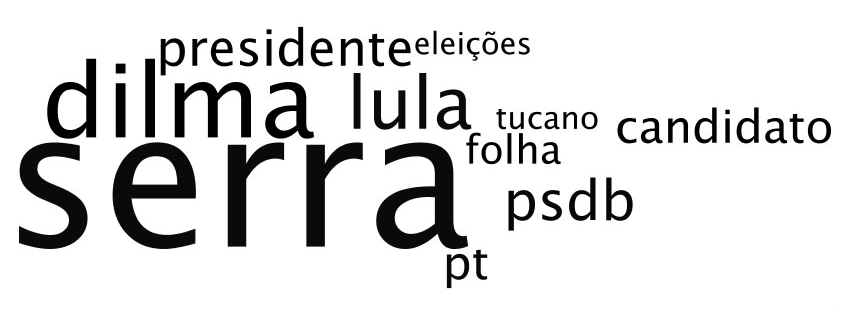
\includegraphics[width=12.5cm, height=6.5cm]{situacao.png}\\
  \caption{Representação gráfica para as dez palavras associadas ao tópico pró-situação na Tabela 4.3.}
  \label{situacao}
\end{figure}

\begin{figure}[h]
  \centering % este comando é usado para centralizar a Figura
  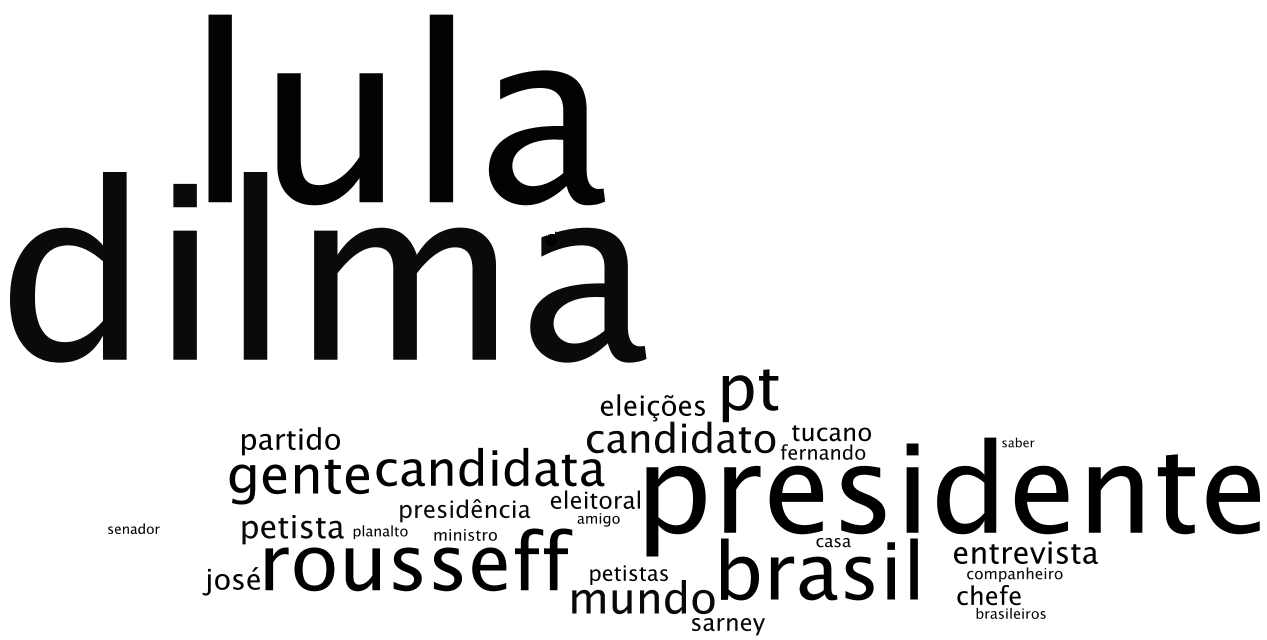
\includegraphics[width=12.5cm, height=6.5cm]{oposicao.png}\\
  \caption{Representação gráfica para as dez palavras associadas ao tópico pró-oposição na Tabela 4.3.}
  \label{oposicao}
\end{figure}



\begin{figure}[h]
  \centering % este comando é usado para centralizar a Figura
  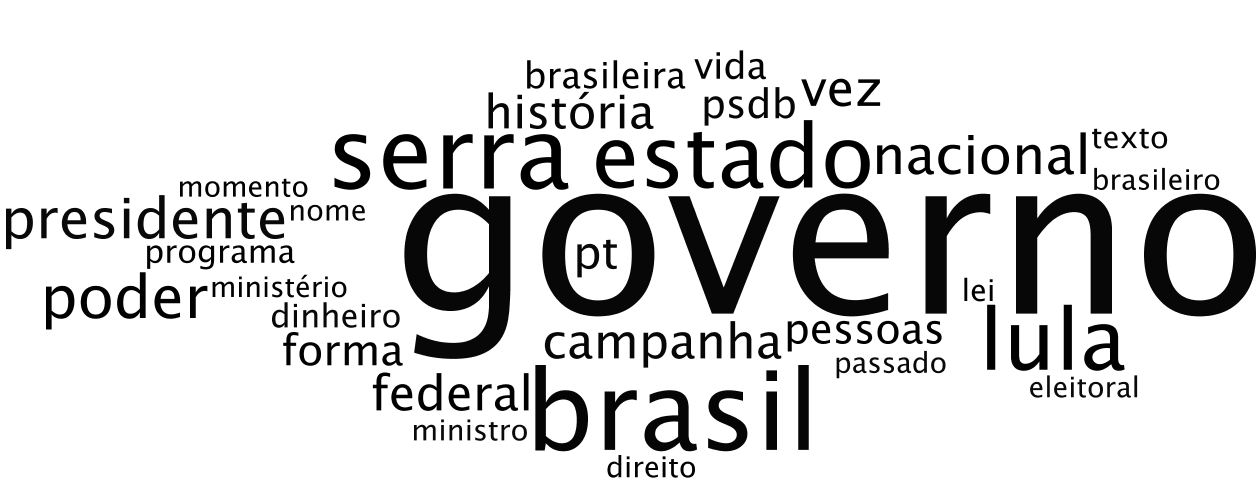
\includegraphics[width=12.5cm, height=6.5cm]{generico.png}\\
  \caption{Representação gráfica para as dez palavras associadas ao tópico genérico na Tabela 4.3.}
  \label{generico}
\end{figure}

Essas figuras também sugerem que os artigos pró-situação dão mais enfoque a personalidades relacionadas à situação, como Lula e Dilma Rousseff, do que os pró-oposição a personalidades da oposição, como José Serra ou Marina Silva. Essa última, inclusive, candidata à presidência pelo PV, não foi mencionada nas palavras listadas na Tabela 4.3. Essas duas observações evidenciam que os veículos, no período analisado, concentraram seus antagonismos em personalidades políticas dos partidos PT, como Lula e Dilma Rousseff, e PSDB, como José Serra.

%É válido ressaltar, por fim, que, apesar dos textos terem caráter crítico e não necessariamente informativo, as palavras elencadas na Tabela 4.3 não carregam uma polaridade natural, como no caso dos adjetivos \emph{bom} ou \emph{ruim}. Isso reforça a ideia de que a expressão de pontos de vista não é tão simples quanto a emissão de opiniões pontuais e claramente polarizadas, como \emph{Serra é um candidato ruim} ou \emph{Lula é um presidente bom}. 

Os pontos de vista desse corpus são construídos através de argumentações complexas, como indicam os trechos de artigos apresentados na seção \ref{estudo:sec1}. Para compreender melhor a relação que as palavras da Tabela 4.3 estabelecem com eles, recomenda-se, por fim, a leitura de um número razoável de passagens de texto que as contenham. Alguns trechos foram selecionados abaixo, em caráter ilustrativo:

\begin{quote}
\emph{"O que parece estarrecedor para quem nunca ouviu \textbf{Dilma} antes - e tenho colegas jornalistas que nunca a viram discursando ou dando \textbf{entrevista} - é absolutamente familiar para os frequentadores desta coluna. Que há nove meses têm acesso a veementes indícios, há muito transformados em provas documentais, de que \textbf{Dilma} é uma afronta imposta ao \textbf{Brasil} por \textbf{Lula}, num [sic] crime lesa-pátria sem perdão."}

{\small Retirado de "O som perturbador do neurônio em ebulição", da coluna de Augusto Nunes - 20/07/2010}
\end{quote}

\begin{quote}
\emph{"Que o \textbf{tucano} \textbf{José} Serra se saiu muito melhor no \textbf{Jornal} Nacional e que a eleição é, sim, de continuidade — no sentido de que não cabe mais falar em ruptura. E fiz uma crítica ou outra ao governo \textbf{Lula}."}

{\small Retirado de "A cabeça dos brasileiros... autoritários", do \emph{blog} de Reinaldo Azevedo - 15/08/2010}
\end{quote}

\begin{quote}

\emph{"A última bala na agulha do \textbf{Serra} é a baixaria. Só que, na era da internet, a baixaria – Lunus (para desconstruir Roseana Sarney) e aloprados do \textbf{PT} (para mandar as ambulâncias superfaturadas para o Inferno) – não tem o mesmo efeito do passado.É o caso dos aloprados do tal dossiê que ele vai ter que explicar na Justiça."}

{\small Retirado de "Serra só tem uma saída: pendurar FHC no pescoço", do \emph{site} Conversa Afiada - 07/06/2010}
\end{quote}

\begin{quote}
\emph{"A entrevista de \textbf{Dilma} ao JN foi didática: \textbf{Dilma} conseguiu colar sua \textbf{candidatura} como continuidade das políticas do governo \textbf{Lula}. Ponto pra ela.Por outro lado, o casal número um do JN da \textbf{Globo} escorregou e mostrou claramente contra quem trabalham em 2010 e a favor de quem se esforçam para mudar tudo o que está aí."}

{\small Retirado de "O povo não é (mais) bobo...", do \emph{blog} Luis Nassif Online - 10/08/2010}
\end{quote}



\chapter{Conclusão}
\label{conclusoes}

Com a disseminação da Web, a elaboração e disseminação de textos carregados com um ponto de vista se popularizou. Não se tratam de documentos que trazem opiniões pontuais a respeito de um único objeto, como um filme ou um livro, mas sim a exposição de argumentos e ideias que, unidos, transmitem a defesa de uma posição a respeito de um certo tema. Enquanto opiniões envolvem um léxico mais restrito, composto de termos como \emph{bom} ou \emph{chato}, as palavras utilizadas na expressão de pontos de vista variam bastante de um tema para outro. Isto dificulta a construção de um conjunto de treinamento que se adeque bem a uma gama variada de temas e é, possivelmente, o principal motivo pelo qual ainda não foi desenvolvida nenhuma ferramenta voltada para pontos de vista genérica para \emph{qualquer tema}. 

Ainda assim, a demanda por entender como as pessoas se posicionam ideologicamente - e em larga escala - existe, e tem fomentado um número crescente de estudos voltados para temáticas específicas. Os artigos revisados no Capítulo \ref{chap3} indicam que a classificação por ponto de vista é mais aplicada a \emph{datasets} que envolvem posicionamentos políticos e temáticas polêmicas, como pena de morte. A leitura da \emph{survey} de Pang e Lee e de alguns artigos sugere, por sua vez, que a classificação por opiniões tem sido mais explorada em \emph{datasets} que envolvem produtos ou serviços \cite{omsa, thumbs-up, peanut-gallery}.

A revisão apresentada no Capítulo \ref{chap3}, além de indicar preferências temáticas na área, também aponta algumas predileções metodológicas. A maioria dos trabalhos classifica os documentos com um Naïve Bayes ou um SVM. Em boa parte dos casos, essa classificação explora apenas as diferentes contagens de palavras nos documentos. Alguns outros artigos exploram propriedades sintáticas ou semânticas dos \emph{datasets} analisados. Outros, por fim, consideram as interações entre os documentos na determinação de seus pontos de vista. A contagem de palavras, simples de ser computada em qualquer língua, foi a característica mais estudada pelos trabalhos revisados - ainda que não tenha recebido destaque em todos eles. Em boa parte dos casos, seu uso exclusivo já é suficiente para uma boa classificação. Em alguns outros, o uso de outras estratégias, mais complexas, foi fundamental para a melhoria na classificação. Diante disso, recomenda-se, inicialmente, para o problema de classificação por ponto de vista, o uso \emph{exclusivo} de contagens de palavras. Se os resultados obtidos não forem satisfatórios, recomenda-se a escolha de um subconjunto ótimo de palavras, como indica o trabalho de Durant e Smith \cite{durant-smith}. Apenas se não houver melhorias significativas, recomenda-se o uso de outras características, um pré-processamento de documentos mais refinado ou a investigação das interações entre os documentos. Essas recomendações, portanto, partem das ideias mais simples para as mais complexas, evitando esforços desnecessários. 
%INTERNACIONALIZÁVEEEEEL!!
%o uso de um pré-processamento mais refinado dos documentos ou 

%Contagens de palavras foram exploradas por muitos artigos, como características diferenciadoras de pontos de vista. De fato, a classificação baseada em contagens de palavras, ou em alguma de suas variações (como a presença/ausência de palavras), assume uma hipótese defendida em estudos de Linguística de corpus: a quantidade de vezes que uma palavra é mencionada em um documento (sua contagem) está diretamente relacionada a quais ideias ele destaca \cite{teubert}. Como consequência, ela funciona melhor em \emph{datasets} nos quais o emprego de palavras varia significativamente por perspectiva. A fim de investigar como o uso de palavras, refletido em suas contagens, se associa ao desempenho da classificação, o Capítulo \ref{chap3} apresenta alguns experimentos neste sentido. Dois corpora são classificados com um Naïve Bayes baseado em contagens de palavras. Via validação cruzada, as taxas de acerto obtidas foram, respectivamente, de 86.22\% e 54.01\%. Isso significa que, no primeiro corpus, as contagens de palavras foram suficientes para identificar corretamente a classe dos documentos de forma satisfatória; no segundo corpus, tem-se o caso contrário. Em outras palavras, isso significa que, no primeiro corpus, o emprego de palavras varia significativamente por perspectiva; no segundo, não. 

%A fim de verificar quais palavras foram mais enfocadas por cada ponto de vista, ampliando a compreensão dos resultados obtidos com o Naïve Bayes, foram feitos experimentos com o modelo L-LDA\footnote{O L-LDA é apresentado no Capítulo \ref{basicos}.}. O modelo associa palavras a tópicos, facilitando a visualização de quais são mais relevantes para cada um deles. Nesses experimentos, cada perspectiva de cada \emph{dataset} corresponde a um tópico, e um último tópico, neutro, é associado a todos os documentos. A finalidade do tópico neutro é filtrar palavras muito comuns em cada corpus, independentemente de perspectiva. Com isso, evidencia-se quais palavras receberam mais destaque por cada perspectiva. Selecionando-se as dez palavras mais frequentemente associadas a cada perspectiva, já é possível visualizar que, no primeiro corpus, perspectivas diferentes enfatizam ideias mais distintas do que no segundo corpus. Isso amplia a compreensão das classificações feitas com o Naïve Bayes, apresentando cenários em que o uso exclusivo de contagens de palavras é ou não suficiente para uma boa classificação. É importante frisar que não se encontrou nenhum outro trabalho que faça uso de um L-LDA para compreender, ainda que parcialmente, como certos termos são enfocados por diferentes perspectivas.

Aproveitando as revisões e análises apresentadas no Capítulo \ref{chap3}, decidiu-se fazer um estudo de caso envolvendo um \emph{dataset} brasileiro. É válido ressaltar que não foi encontrado nenhum outro trabalho que classifique documentos, escritos em português do Brasil, de acordo com seus pontos de vista. Considerando que 2010 é ano de eleições presidenciais no Brasil, a abundância de artigos que carregam pontos de vista típicos da oposição e da situação foi explorada. Foi construído um corpus sobre o atual governo e as eleições, composto de material coletado em colunas, \emph{sites} e \emph{blogs} mantidos por jornalistas de notoriedade nacional. Em seguida, esse corpus foi dividido entre os pontos de vista pró-situação e pró-oposição, e foi classificado com um Naïve Bayes. As características dos documentos exploradas por esse classificador foram suas contagens de palavras. Os resultados obtidos com essa metodologia foram muito positivos: a taxa de acerto, em particular, foi de 89.43\%. Isso significa que esses jornalistas consolidam suas perspectivas sobre a política brasileira já nas palavras que destacam. De fato, alguns trechos elencados no Capítulo \ref{estudo}, no qual o estudo é apresentado, sugerem que seus pontos de vista são defendidos com muita veemência. 

Esse estudo de caso também investiga quais palavras receberam mais destaque por cada ponto de vista. A análise com um L-LDA, associando cada ponto de vista a um tópico e um tópico neutro a todos os documentos, indica que os jornalistas pró-situação dão mais ênfase ao candidato de oposição José Serra do que os pró-oposição. Esses últimos, por sua vez, dão maior destaque ao presidente Lula e à sua candidata, Dilma Rousseff - ambos correspondem à situação. Isso sugere que os jornalistas enfatizam o ataque aos candidatos que se opõem, ideologicamente, aos pontos de vista que eles defendem. Isso reforça a ideia, empiricamente observável, de que a defesa de um posicionamento, muitas vezes, compreende o ataque a posicionamentos opostos, como sugerem Somasundaran e Wiebe em seu trabalho sobre debates \emph{online} \cite{wiebe}.  
%, assim como no Capítulo \ref{chap3},
%cado de forma semelhante àquela do Capítulo \ref{chap3}, 

\section{Dificuldades encontradas}

A classificação de documentos de acordo com seus pontos de vista sobre um tema é um problema relativamente novo. De fato, ele só foi estabelecido como sub-área da Mineração de Opinião em 2008, na \emph{survey} de Pang e Lee. Por este motivo, para entender melhor o problema, foi necessário buscar artigos em diversas conferências que envolviam a área de Mineração de Opinião. A filtragem de quais resultados realmente tinham a ver com o tema dessa monografia não foi exatamente difícil, mas envolveu um trabalho manual considerável. Para o estudo de caso, a extração, filtragem e padronização dos documentos que compõem o corpus também envolveu algum trabalho manual. Embora essas tarefas tenham sido realizadas de forma automatizada, a construção dos \emph{scripts} dependia da compreensão de como o conteúdo estava disposto em cada veículo.  

\section{Trabalhos futuros}

Futuramente, pretende-se estender o estudo de caso do Capítulo \ref{estudo} a textos políticos escritos por cidadãos comuns em seus \emph{blogs}, o que pode contribuir positivamente para a compreensão de como o brasileiro se posiciona politicamente na Web. Além disso, o estudo também deve ser ampliado para identificar os pontos de vista contidos nos comentários feitos aos artigos do corpus, em seus \emph{blogs}, \emph{sites} e colunas, a fim de se avaliar como eles refletem o posicionamento dos leitores em relação àquilo que leram. Este tipo de análise pode ajudar a compreender o impacto destes artigos em seus leitores e a formação de posicionamentos na mídia brasileira \emph{online}. Caso essas tarefas de classificação não sejam bem resolvidas com o uso exclusivo de contagens de palavras, esforços direcionados na busca de características mais complexas, envolvendo aspectos sintáticos/semânticos dos documentos, devem ser feitos. É válido ressaltar que isso provavelmente implicaria no desenvolvimento de ferramentas gramaticais de apoio, voltadas para a língua portuguesa.




\bibliography{monografia}
\appendix

\chapter{Teorema de Bayes e notações}

A Estatística se alia à Teoria da Probabilidade para estimar e analisar a ocorrência de eventos, como \emph{Ganho de cem reais em sorteio} ou \emph{Chuva ao meio-dia}. Dados dois eventos \emph{A} e \emph{B}, temos que a probabilidade \emph{a priori} de \emph{A} acontecer \textbf{ignora} a ocorrência do evento \emph{B}. Essa probabilidade é representada pela notação \ensuremath{P(A)}. Analogamente, para o evento \emph{B}, tem-se \ensuremath{P(B)}. Na prática sabe-se, intuitivamente, que a ocorrência de determinados eventos interfere no acontecimento de outros. Se às onze e meia da manhã observa-se o evento \emph{Céu nublado}, a probabilidade do evento \emph{Chuva ao meio-dia} ocorrer pode diferir daquela que ignora esse primeiro evento. Neste sentido, a probabilidade de um evento \emph{A} ocorrer \emph{dado} que \emph{B} ocorreu recebe o nome de probabilidade \emph{a posteriori} de \emph{A} condicional a \emph{B}, e é denotada por \ensuremath{P(A\mbox{ }|\mbox{ }B)}. Analogamente, tem-se \ensuremath{P(B\mbox{ }|\mbox{ }A)}. O Teorema de Bayes correlaciona essas probabilidades da seguinte forma 

\begin{equation}
\label{bayes-apendice}
\ensuremath{P(A\mbox{ }|\mbox{ }B) = \frac{P(B\mbox{ }|\mbox{ }A)P(A)}{P(B)}} 
\end{equation}

O classificador Naïve Bayes se baseia em uma aplicação direta do Teorema de Bayes. Dados os eventos \emph{Obtenção de um documento x} e \emph{Obtenção de uma classe y}, o classificador deve estimar a ocorrência do segundo evento assumindo que o primeiro já ocorreu.   



\end{document}

